\section{Tracking by Inverse Rendering }\label{sec:method}
% \noindent
We cast object tracking as a test-time inverse rendering problem that fits generated multi-object scenes to the observed image frames. First, we discuss the proposed scene representation we fit. Next, we devise our rendering-based test-time optimization at the heart of the proposed tracking approach.
We employ an object-centric scene representation. We model the underlying 3D scene for a frame observation as a composition of all object instances without the background scene.

\subsection{Scene Generation}

% \vspace{0.5\baselineskip}
\noindent \textbf{Object Prior.}  To represent a large, diverse set of instances per class, we define each object instance $o$ as a sample from a distribution $\boldsymbol{O}$ over all objects in a class, that is
\vspace*{-6pt}
\begin{equation}
    \boldsymbol{O} \sim f\left(\boldsymbol{o}\right)\text{,}
\end{equation}
where $f$ is a learned function over a known prior object distribution. Here, the prior distribution is modeled by a differentiable generative 3D object model $o_p = G\left(z_p\right)$, that maps a latent embedding $z_p$ to an object instance $o_p$, the object $p$. In particular, the latent space comprises two disentangled spaces $\boldsymbol{z}_S$ and $\boldsymbol{z}_T$ for shape $S$ and texture $T.

Given an object-centric camera projection $\mathbf{P}_c = \mathbf{K}_c \mathbf{T}$, where $\mathbf{K}_c $ is the camera intrinsic matrix, a transformation $\mathbf{T} = \left[ \mathbf{R} | \mathbf{t} \right]$ to camera $c$ that is composed of rotation $\mathbf{R}$ and translation $\mathbf{t}$, a differentiable rendering method $R\left(o_p, c\right)$, such as rasterization for meshes or volumetric rendering for neural fields, this renders an image $I_{c,p}$, a 2D observation of the 3D object $o_p$. While our method is general, implementation details of the generator and rendering method are provided in the implementation section.

\vspace{0.5\baselineskip}
\noindent \textbf{Scene Composition.} We model a multi-object scene as a scene graph composed of transformations in the edges and object instances in the leaf nodes, similar to Ost \emph{et al.}~\cite{ost2021neural}. Object poses are described by the homogeneous transformation matrix $\mathbf{T}_{p} \in \mathbb{R}^{4x4}$ with the translation $\mathbf{t}_{p}$ and orientation $\mathbf{R}_{p}$ in the reference coordinate system. The camera pose $\mathbf{T}_{c} \in \mathbb{R}^{4x4}$ is described in the same reference coordinate system. The relative transformation of the camera $c$ and each object instance $p$ can be computed through edge traversal in the scene graph as
% \vspace*{-8pt}
\begin{equation}\label{eq:camera_to_obj}
    \mathbf{T}_{c,p} = \text{diag}\left(\frac{1}{s_{p}}\right)\mathbf{T}_{p}\mathbf{T}_{c}^{-1},
\end{equation}
%
where the factor $s_{p}$ is a scaling factor along all axes to allow a shared object representation of a unified scale. This canonical object scale is necessary to represent objects of various sizes, independent of the learned prior on shape and texture. The object centric projection $\mathbf{P}_{c,p} = \mathbf{K}_c \mathbf{T}_{c,p} $ is used to render the RGB image $I_{c,p} \in \mathcal{R}^{H \times W \times 3}$ and mask $M_{c, p} \in \left[0, 1 \right]^{H \times W}$ for each object/camera pair. 

Individual rendered RGB images are ordered by object distance $\| \mathbf{t}_{c, p} \|$, such that $p=1$ is the shortest distance to $c$. Using the Hadamard product of the non-occluded mask $\gamma_p$ all $N_o $, object images are composed into a single image
% \vspace*{-8pt}
\begin{equation}\label{eq:forward_scene}
    \begin{aligned}
            \hat I_c &= \sum_{k = 1}^{N_o} R\left( G\left( \mathbf{z}_{S,p}, \mathbf{z}_{T,p} \right), \mathbf{P}_{c,p}\right) \circ \mathbf{\gamma}_p, \text{\,\,where  } \\        
             \mathbf{\gamma}_p  & = \max \left( \left( \mathbf{M}_{c, p} - \sum_{q=1}^{p} \mathbf{M}_{c,q} \right), \mathbf{0}^{H\times W} \right),
    \end{aligned}
\end{equation}
where instance masks are generated in the same fashion. 

\subsection{Inverse Multi-Object Scene Rendering.}\label{ssec:scene_rep}
%
% \noindent
We invert the differentiable rendering model defined in Eq.~\ref{eq:forward_scene} by optimizing the set of all object representations in a given image $I_c$ with gradient-based optimization. We assume that, initially, each object $o_p$ is placed at a pose $\hat{\mathbf{T}}_{c,p}$ and scaled with $\hat s_p$ near its underlying location. We represent object orientations in their respective Lie algebraic form $\mathfrak{so}(3)$. We further sample an object embedding $\hat{\mathbf{z}}_{S,p}$ and $\hat{\mathbf{z}}_{T,p}$ in the respective latent embedding space.


For in-the-wild images, $I_c$ is not just composed of sampled object instances but other objects and the scene background. Since our goal for tracking is the reconstruction of all object instances of specific object classes, a na\"ive $\ell_2$ image matching objective of the form $\| I_c - \hat{I}_c \|_2$ is noisy and challenging to solve with vanilla stochastic gradient descent methods. To tackle this issue, we optimize visual similarity in the generated object regions instead of the full image. We optimize only on rendered RGB pixels and minimize
\begin{equation}\label{eq:loss_mse}
% \begin{aligned}
    \mathcal{L}_{RGB} = \| \left( I_c - \hat{I}_c \right) \circ \hat{M}_{I_c} \|_2, \text{\,\,with\ }\nonumber \hat{M}_{I_c} = \min \left( \sum M_{c,p} , \mathbf{1}\right).
% \end{aligned}
\end{equation}
The mask of all foreground/object pixels $\hat{M}_{I_c}$ is computed as the sum over all object masks $M_{c,p}$ in the frame rendered by camera $c$.
We employ a learned perceptual similarity metric~\cite{zhang2018perceptual} (LPIPS) on object-centered image patches, that is
% \vspace*{-6pt}
\begin{equation}\label{eq:loss_lpips}
    \mathcal{L}_{perceptual} = \text{LPIPS}_{patch}\left( I_c, \hat{I}_{c,p}  \right).
\end{equation}
The combined loss function of our method is
\begin{equation}\label{eq:loss_mse_lpips}
    \mathcal{L}_{IR} = {L}_{RGB} + \lambda \mathcal{L}_{perceptual},
\end{equation}
which we optimize by refining the latent codes of shape and appearance, position, rotation, and scale, leading to
% \vspace*{-6pt}
\begin{equation}
        \hat{\mathbf{z}}_{S,p}, \hat{\mathbf{z}}_{T,p}, \hat{s}_{p} \hat{\mathbf{t}}_p, \hat{\mathbf{R}}_p = \text{arg min} \left( \mathcal{L}_{IR} \right) .
\end{equation}
Instead of using vanilla stochastic gradient descent methods, we propose an alternating optimization schedule of distinct properties that includes aligning $z_S$ before $z_T$, to reduce the number of total optimization steps. A detailed implementation and validation of all design choices of the optimization are presented in the Supplementary Material.

\vspace{0.5\baselineskip} \noindent \textbf{Optimization.}
To solve Eq.~\ref{eq:loss_mse_lpips}, we propose an optimization schedule, that first optimizes a coarse color, and then jointly optimizes the shape and the positional state of each object. As the backbone of the learned perceptual loss, we use a pre-trained VGG16~\cite{simonyan2015deep} and utilize individual output feature map similarities at different points of the optimization. We find that color and other low-dimensional features are represented in the initial feature maps and those are better guidance for texture than high-dimensional features as outputs of the later blocks. These features have a more informative signal for shape and object pose. We use the average of the first and second blocks in the optimization for $\mathbf{z}_T$, while the combined perceptual similarity loss guides the optimization of  $\mathbf{z}_T$ and the pose.

We initialize all object embeddings with the same fixed values inside the embedding space, take two optimization steps solely on color utilizing the described loss, and then freeze the color for the joint optimization of the shape and pose. We regularize out-of-distribution generations with
\begin{equation}\label{eq:regularize}
    \mathcal{L}_{embed} = \alpha_T\mathbf{z}_T + (1 - \alpha_T)\mathbf{z}_T^{avg} +  \alpha_S\mathbf{z}_S + (1 - \alpha_S)\mathbf{z}_S^{avg}
\end{equation}
that minimizes a weighted distance in each dimension with respect to the average embedding  $\mathbf{z}_S$ or $\mathbf{z}_T$ respectively. For optimization, we use the ADAM optimizer \cite{Kingma2015AdamAM}.
The final loss function combines the RGB, perceptual cost \ref{eq:loss_mse_lpips} and the regularization \ref{eq:regularize} with $\lambda=10$, $\alpha_{T}=0.7$ and $\alpha_{S}=0.7$. We freeze color after two steps of optimization and optimize the shape and scale for three more steps, adding translation and rotation only in the last two steps.

\subsection{3D Multi-Object Tracking via Inverse Rendering}
% \noindent
Next, we describe the proposed method for tracking multiple dynamic objects with the inverse rendering approach from above. The approach tracks objects in the proposed representation across video frames and is illustrated in Fig.~\ref{fig:pipeline}. For readability, we omit $p$ and the split of $\mathbf{z}$ into $\mathbf{z}_S$ and $\mathbf{z}_T$ in the following.

\vspace{0.5\baselineskip} \noindent \textbf{Initial Object and Pose Estimation.}
Common to tracking methods, we initialize with a given initial 3D detection on image $I_{c,k}$, and we set object location $\mathbf{t}_{k} = \left[x, y, z\right]_{k}$, scale $s_{k} = \max(\text{w}_{k}, \text{h}_{k}, \text{l}_{k})$ using the detected bounding box dimensions and heading $\psi_{k}$ in frame $k$. We then find an optimal representation $\boldmath{z}_k$, and a refined location and rotation of each object $o$ via the previously introduced inverse rendering pipeline for multi-object scenes. The resulting location, rotation, and scale lead to the observation vector 
% \vspace{-8pt}
\begin{equation}\label{eq:observation}
\mathbf{y}_{k} = [\mathbf{t}_{k}, s_{k},\psi_{k}] .
\end{equation}

\vspace{-16pt}
\vspace{0.5\baselineskip} \noindent \textbf{Prediction.}
%
While not confined to a specific dynamics model, we use a linear state-transition model $\textbf{A}$, for the objects state $\mathbf{x}_{k} = [x, y, z, s, \psi, w, h, l, {x}', {y}', {z}']_{k}$, and a forward prediction using a Kalman Filter~\cite{kalman1960new}, a vanilla approach in 3D object tracking~\cite{weng2020AB3DMOT}. An instantiated object in k-1 can be predicted in frame $k$ as
\begin{equation}
   \hat{\mathbf{x}}_{k|k-1} = \mathbf{A}\hat{\mathbf{x}}_{k-1|k-1} \text{ and } \mathbf{P}_{k|k-1} = \mathbf{A}\mathbf{P}_{k-1|k-1}\mathbf{A}^T + \mathbf{Q}, 
\end{equation}
with the predicted \textit{a priori} covariance matrix modeling the uncertainty in the predicted state.

% \begin{figure*}[t!]
% 	% \vspace{-20pt}
% 	\centering
% 	\resizebox{0.98\linewidth}{!}{
% 	\renewcommand{\arraystretch}{0.5}
% 	\begin{tabular}{@{}c@{\hskip 0.05cm}c@{\hskip 0.05cm}c@{\hskip 0.05cm}c@{\hskip 0.05cm}c@{\hskip 0.05cm}c@{}}
% 		\centering
%             &
% 		{\small Input $t_0$}&
% 		{\small Tracked $t_0$}&
% 		{\small Tracked $t_1$}&
% 		{\small Tracked $t_2$}&
% 		{\small Tracked $t_3$}\\

%             \rotatebox[origin=c]{90}{{\footnotesize	  Suburban}}&
% 		 \raisebox{-0.5\height}{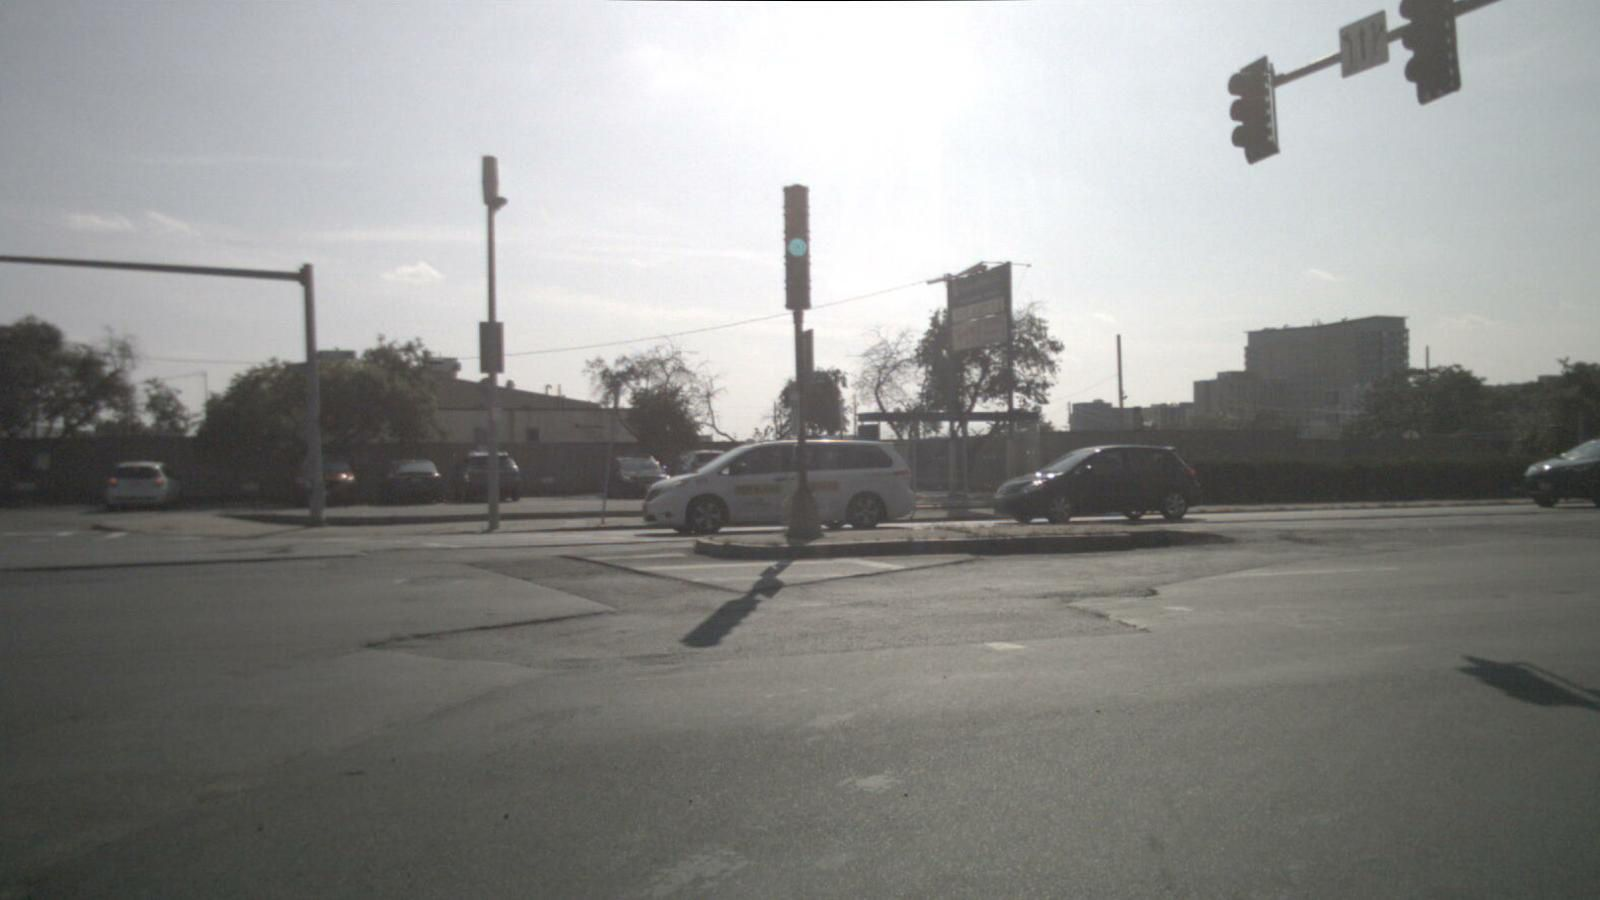
\includegraphics[width=.19\columnwidth, trim={0cm 0cm 0cm 0cm},clip]{fig/nuScenes_main/scene2/0484_2_gt.png}}&
% 		 \raisebox{-0.5\height}{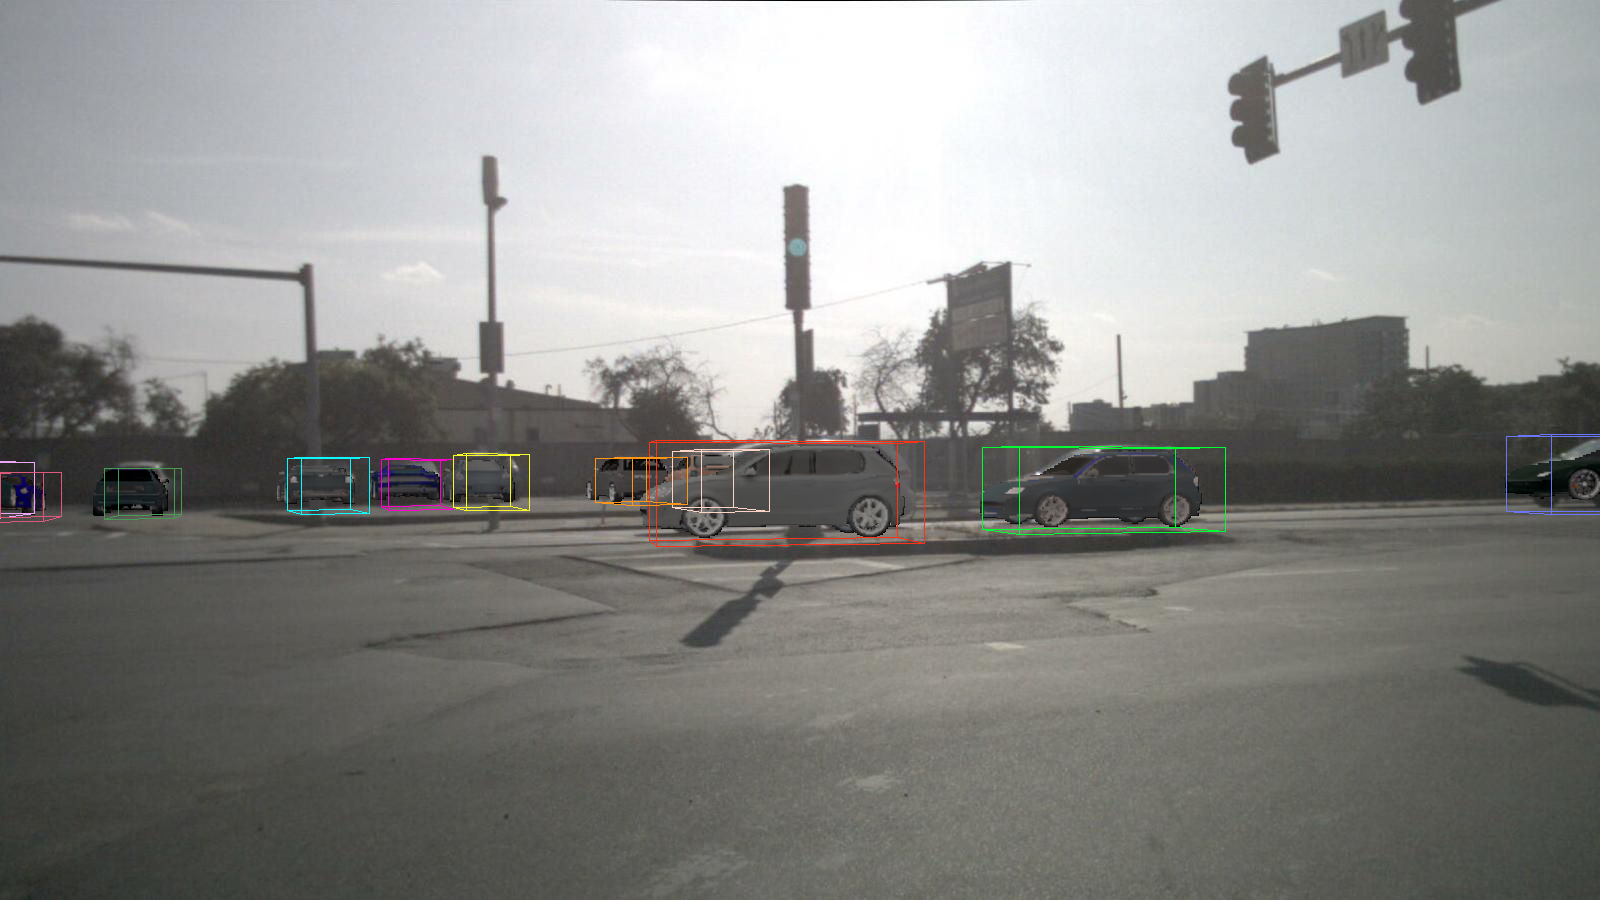
\includegraphics[width=.19\columnwidth, trim={0cm 0cm 0cm 0cm},clip]{fig/nuScenes_main/scene2/0484_2_bbox.png}}&
% 		 \raisebox{-0.5\height}{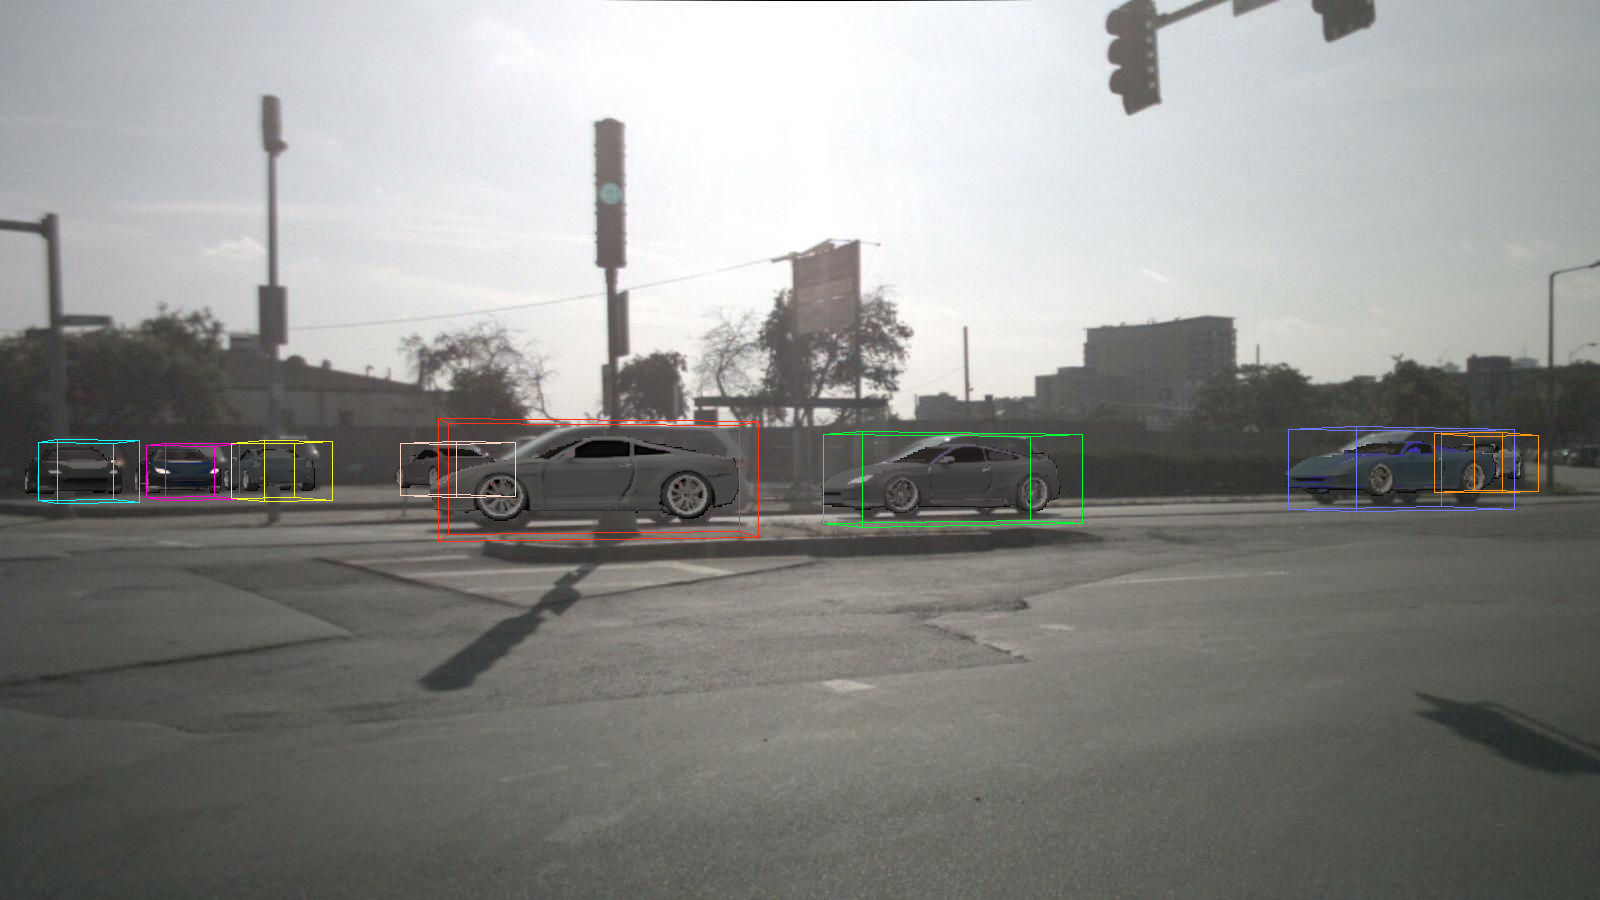
\includegraphics[width=.19\columnwidth, trim={0cm 0cm 0cm 0cm},clip]{fig/nuScenes_main/scene2/0484_3_bbox.png}}&
% 		 \raisebox{-0.5\height}{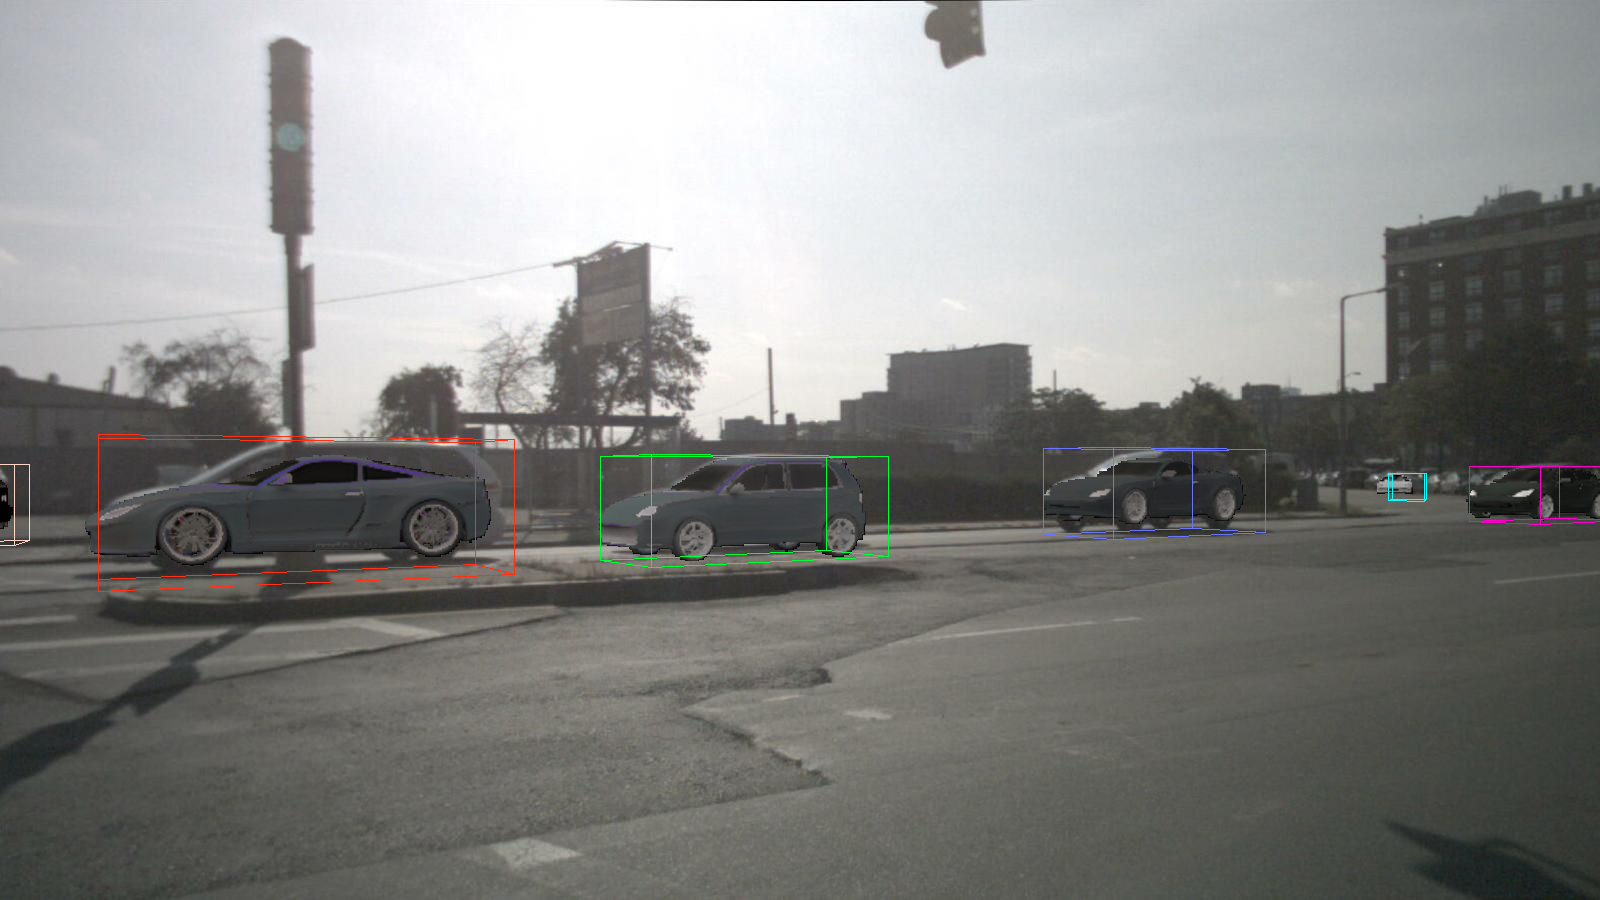
\includegraphics[width=.19\columnwidth, trim={0cm 0cm 0cm 0cm},clip]{fig/nuScenes_main/scene2/0484_4_bbox.png}}&
% 		 \raisebox{-0.5\height}{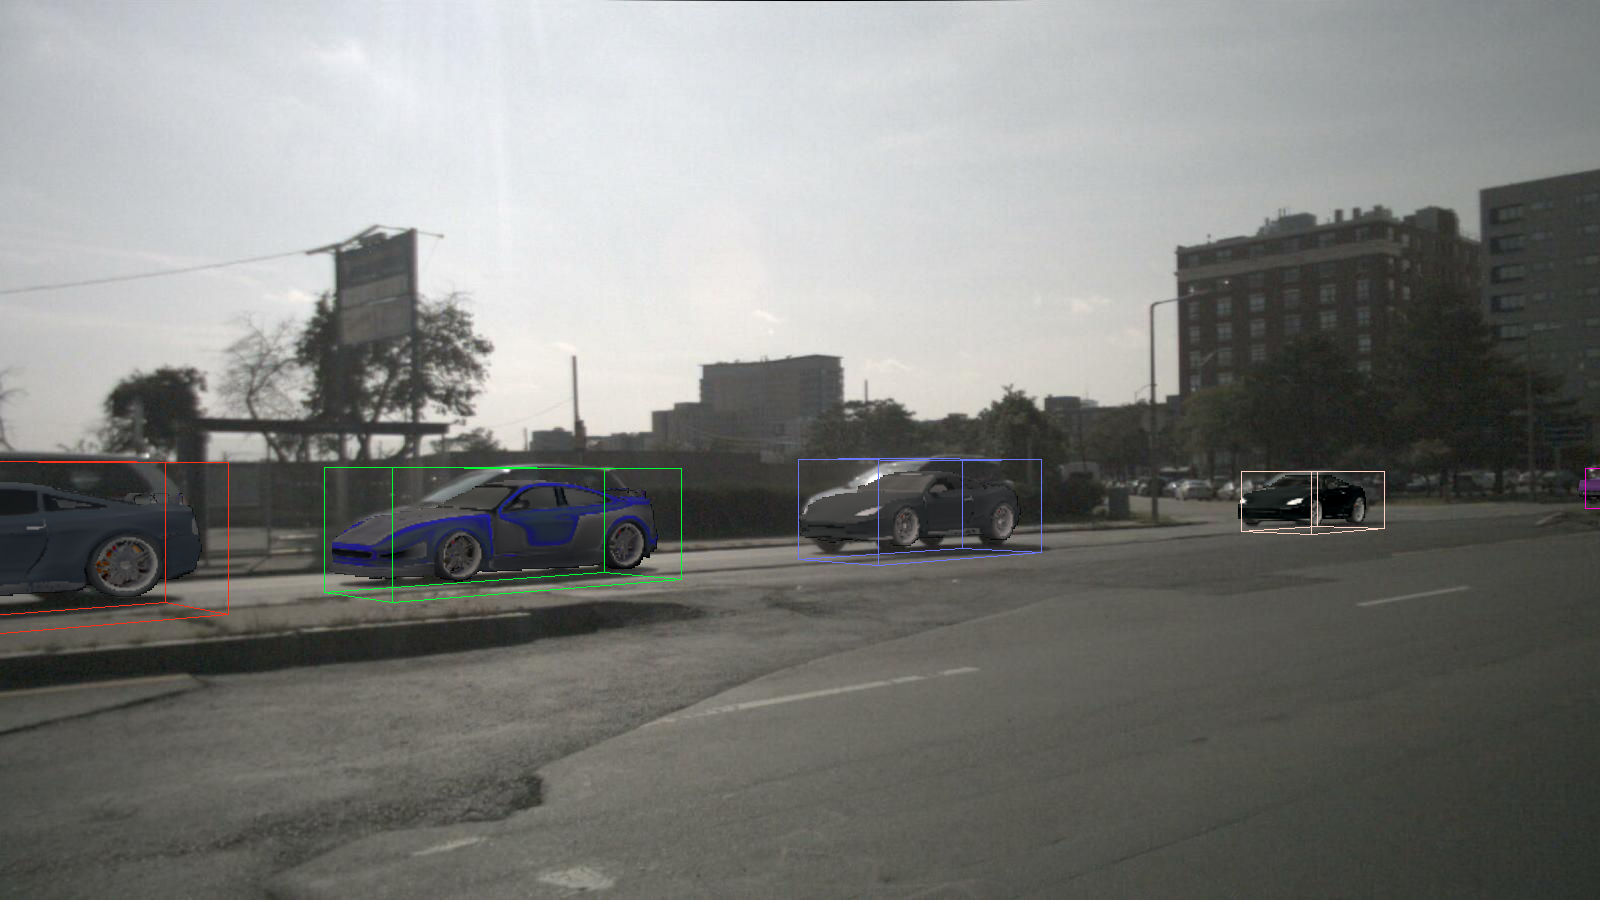
\includegraphics[width=.19\columnwidth, trim={0cm 0cm 0cm 0cm},clip]{fig/nuScenes_main/scene2/0484_5_bbox.png}}\\[0.95cm]
  
% 		\rotatebox[origin=c]{90}{{\footnotesize	 Dense Urban}}&
% 		\raisebox{-0.5\height}{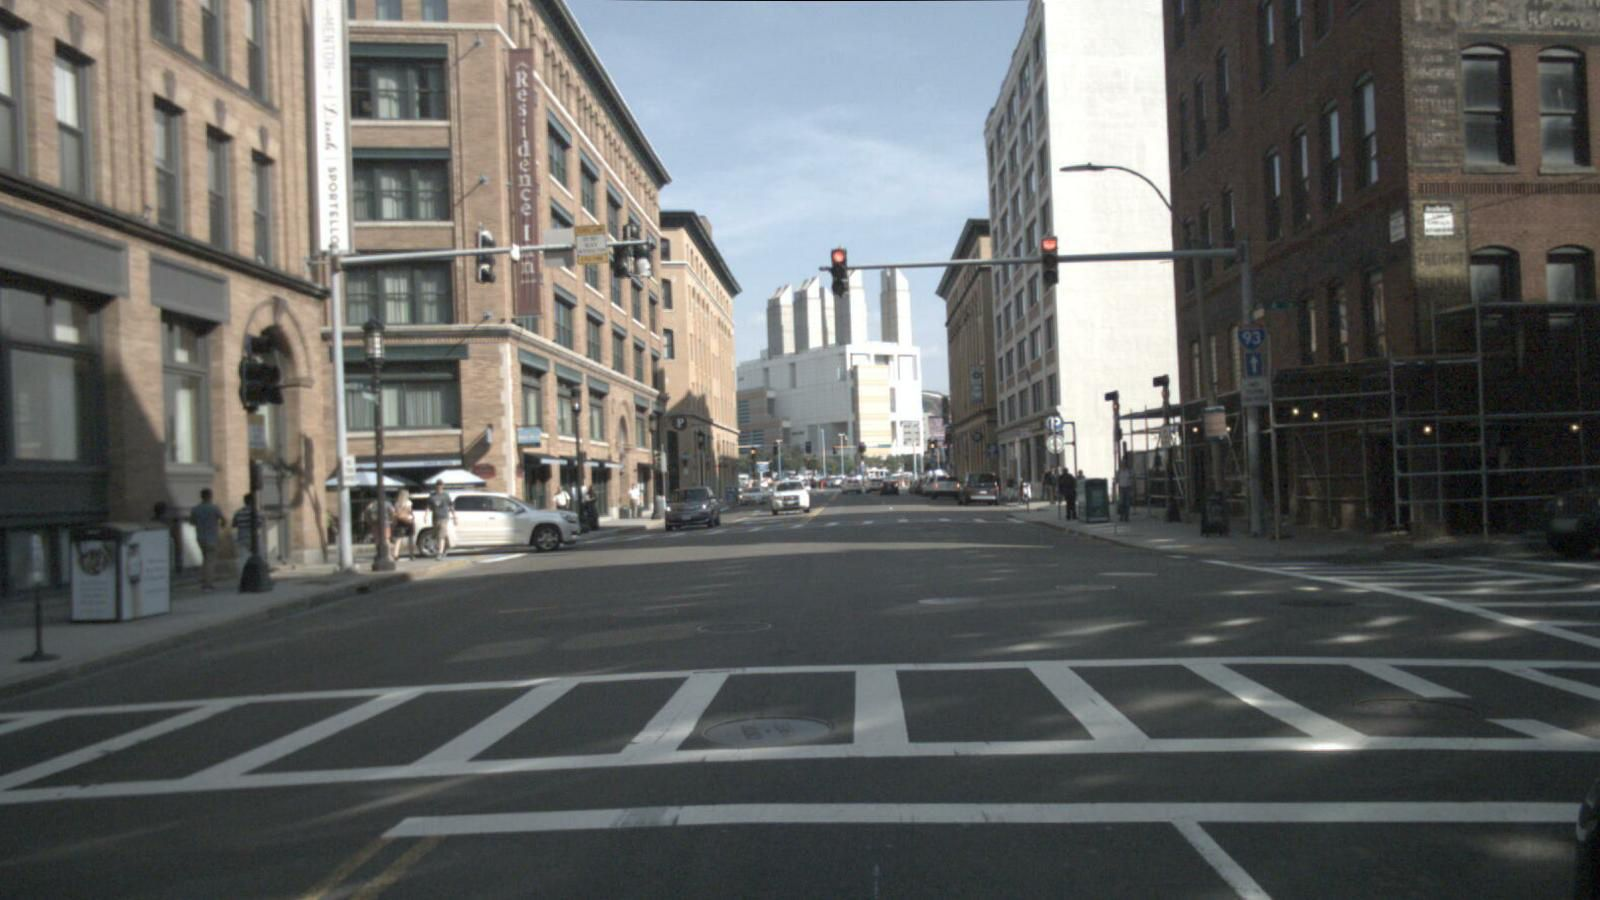
\includegraphics[width=.19\columnwidth, trim={0cm 0cm 0cm 0cm},clip]{fig/nuScenes_main/scene3/0496_30_gt.png}}&
% 		\raisebox{-0.5\height}{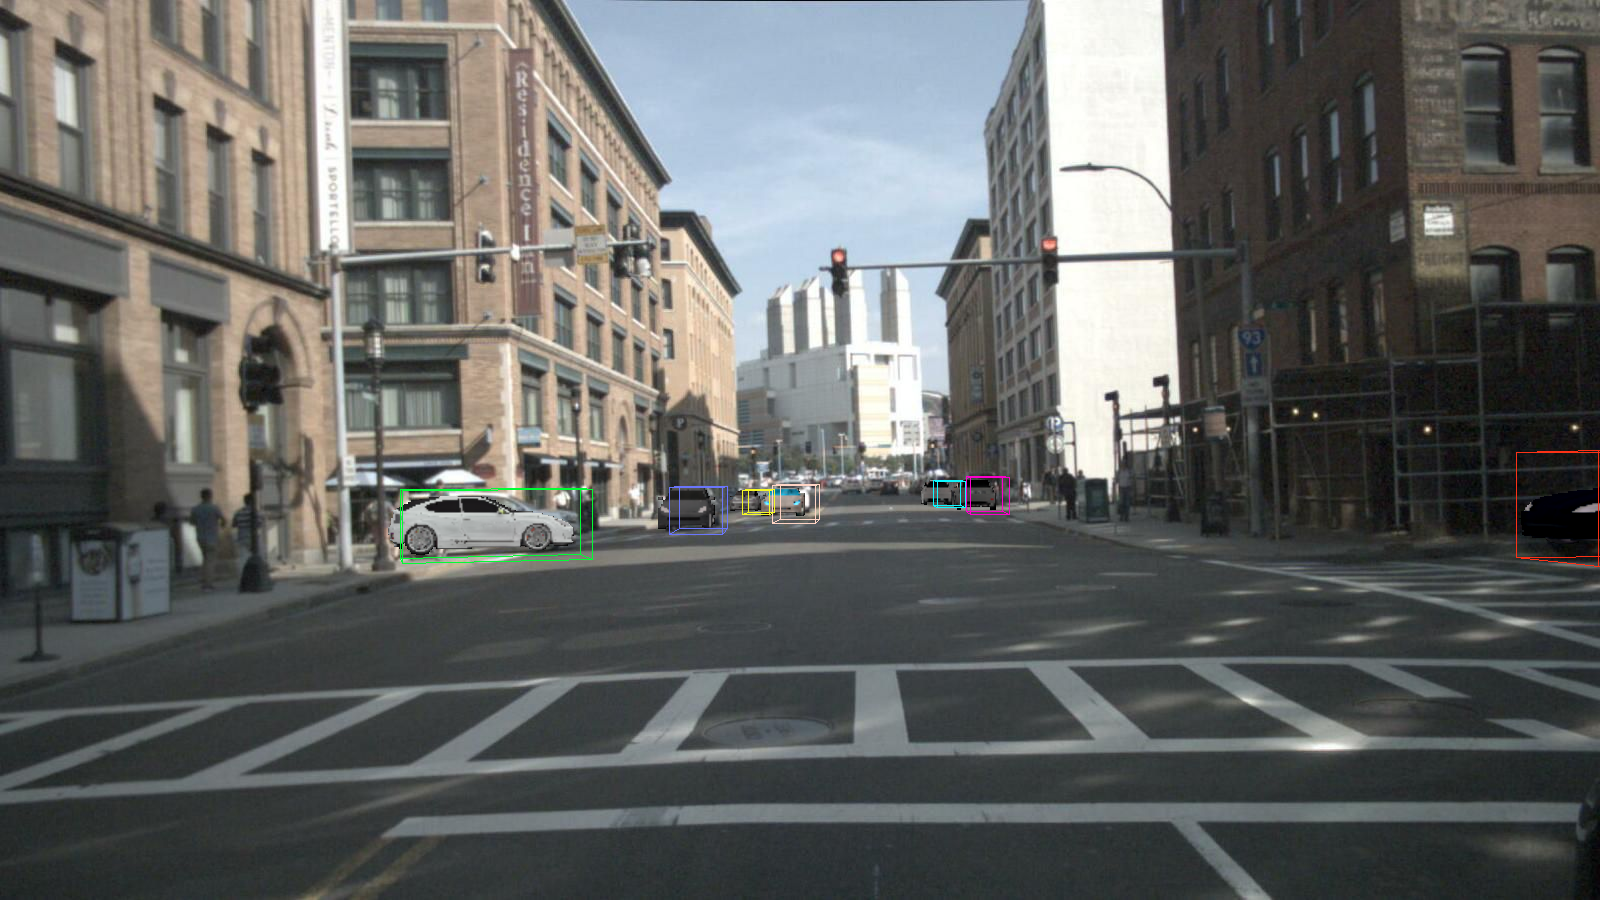
\includegraphics[width=.19\columnwidth, trim={0cm 0cm 0cm 0cm},clip]{fig/nuScenes_main/scene3/0496_30_bbox.png}} &
% 		\raisebox{-0.5\height}{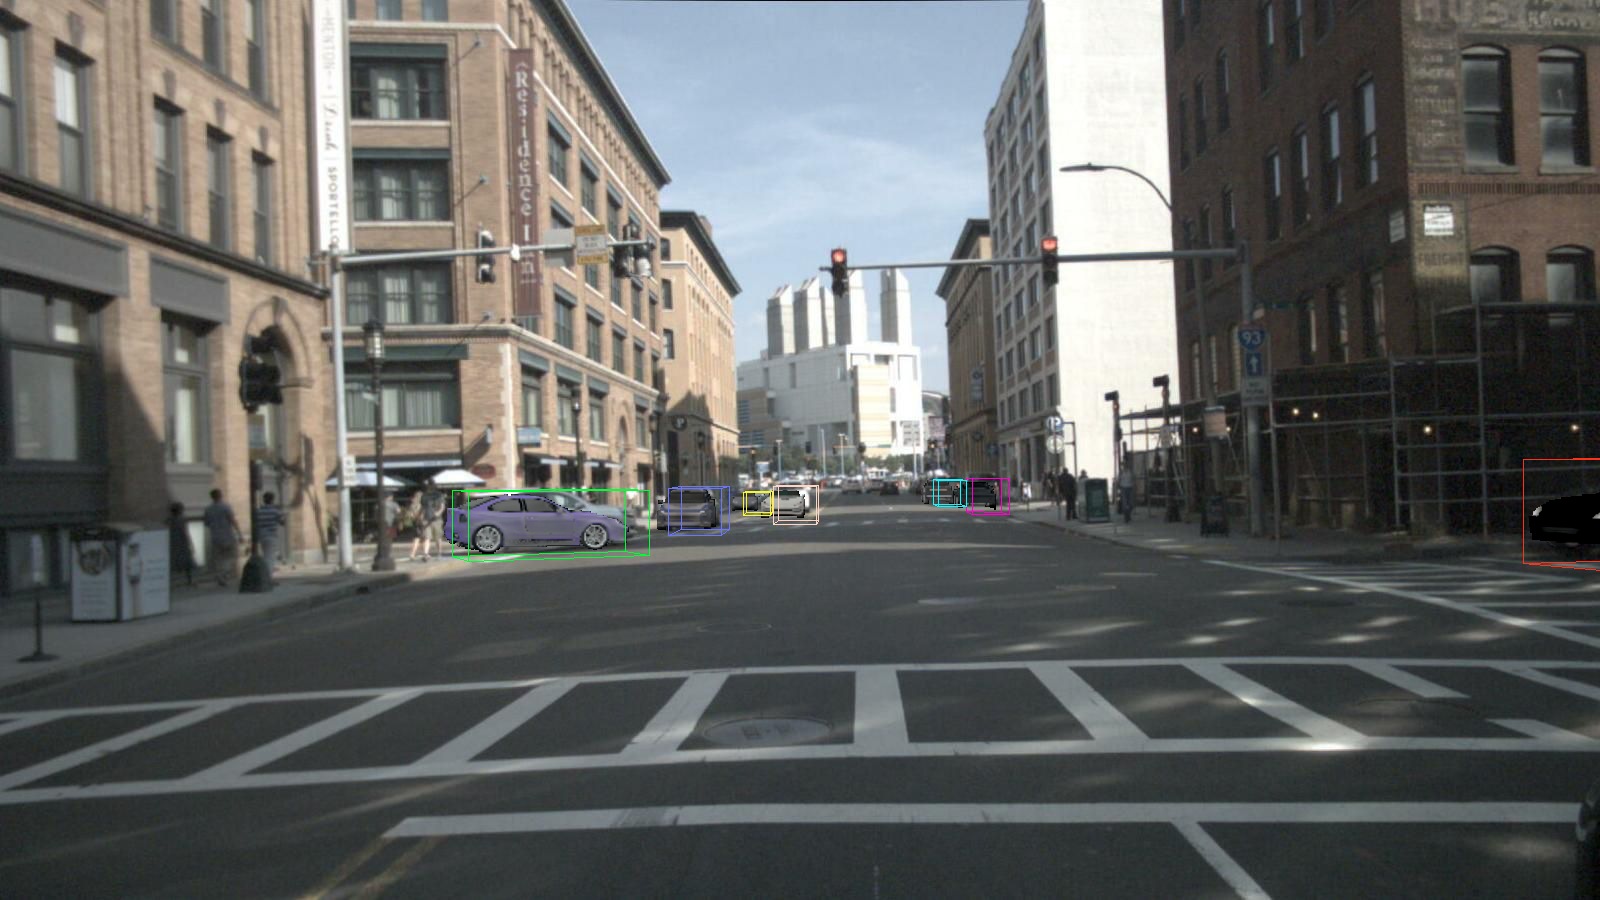
\includegraphics[width=.19\columnwidth, trim={0cm 0cm 0cm 0cm},clip]{fig/nuScenes_main/scene3/0496_31_bbox.png}}&
% 		\raisebox{-0.5\height}{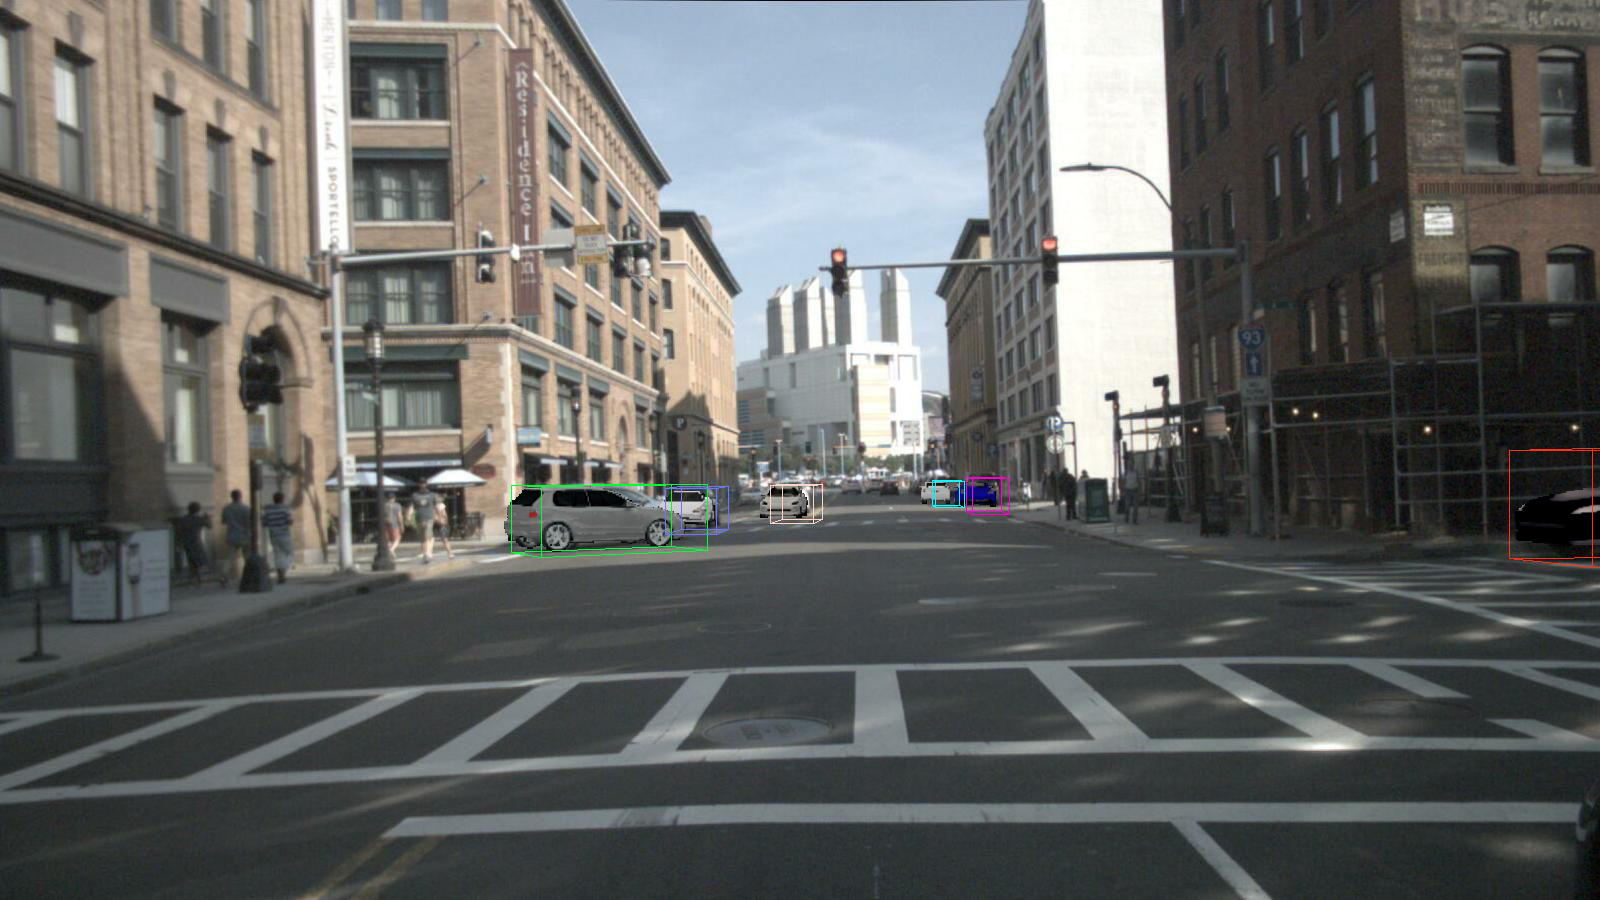
\includegraphics[width=.19\columnwidth, trim={0cm 0cm 0cm 0cm},clip]{fig/nuScenes_main/scene3/0496_32_bbox.png}}&
% 		\raisebox{-0.5\height}{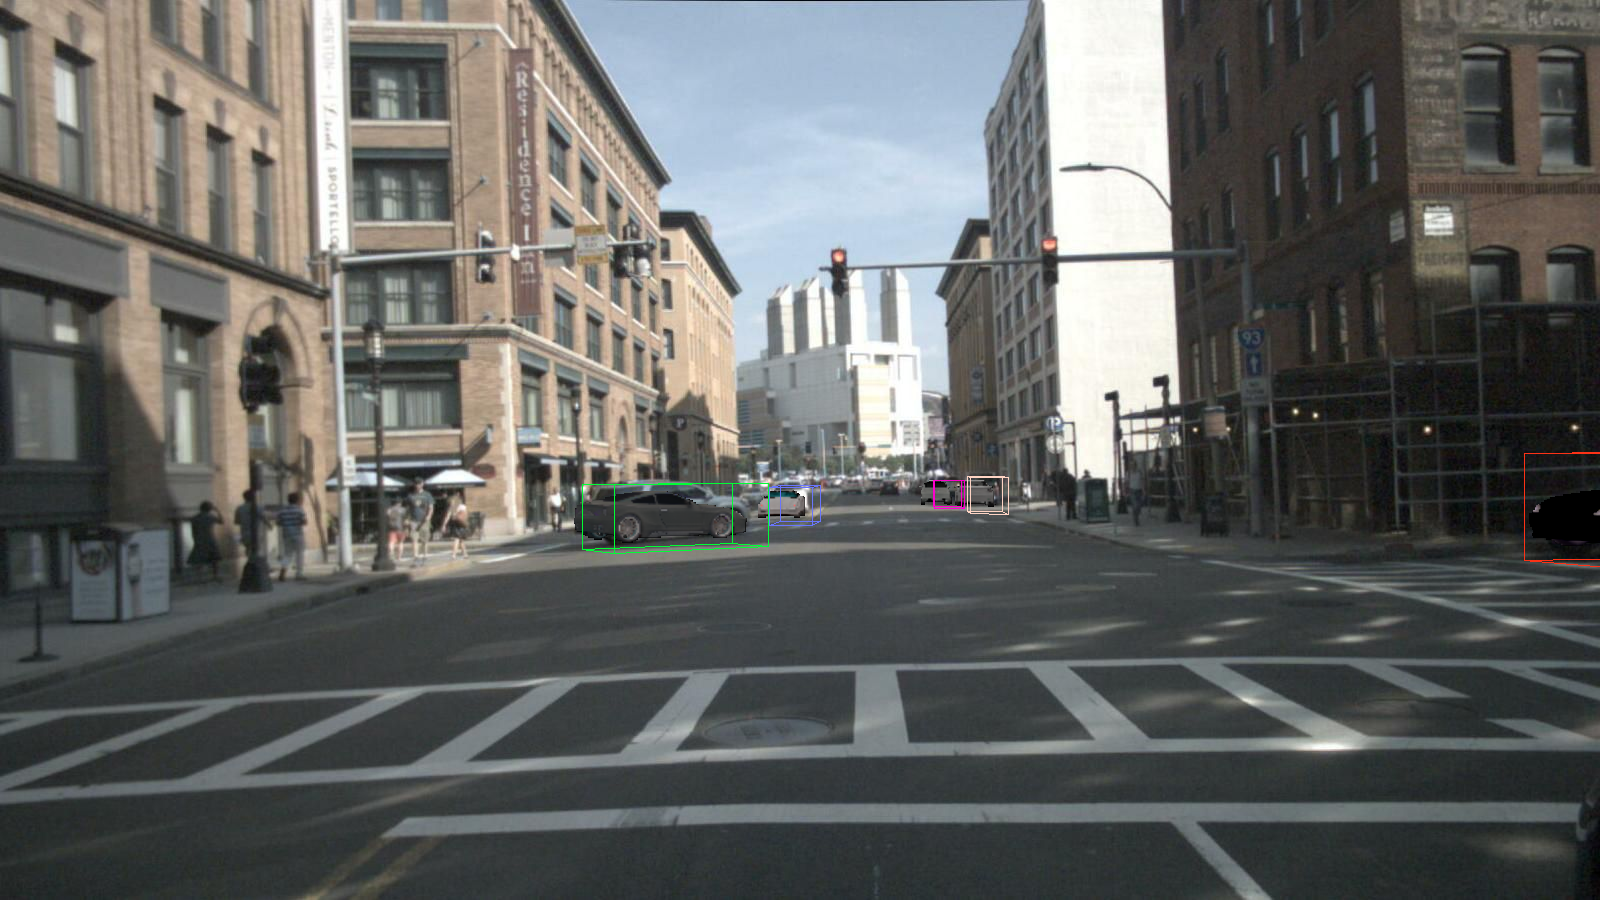
\includegraphics[width=.19\columnwidth, trim={0cm 0cm 0cm 0cm},clip]{fig/nuScenes_main/scene3/0496_33_bbox.png}}\\[0.7cm]
  
%             \rotatebox[origin=c]{90}{{\footnotesize	 Clutter}}&
%   		\raisebox{-0.5\height}{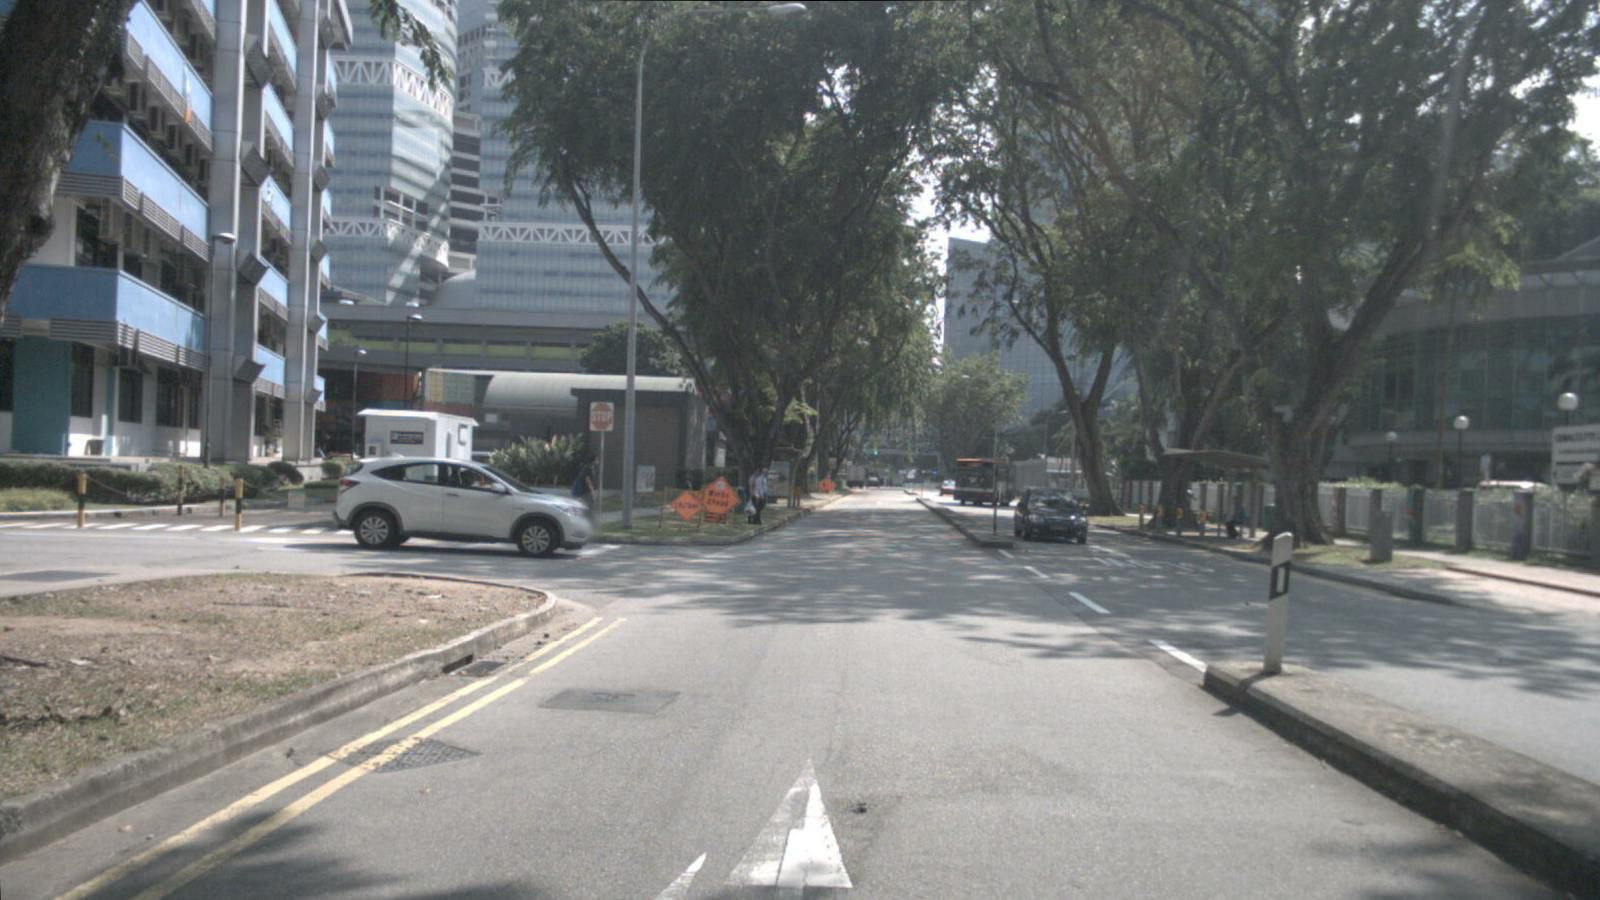
\includegraphics[width=.19\columnwidth, trim={0cm 0cm 0cm 0cm},clip]{fig/nuScenes_main/scene6/28_gt_img.png}}&
% 		\raisebox{-0.5\height}{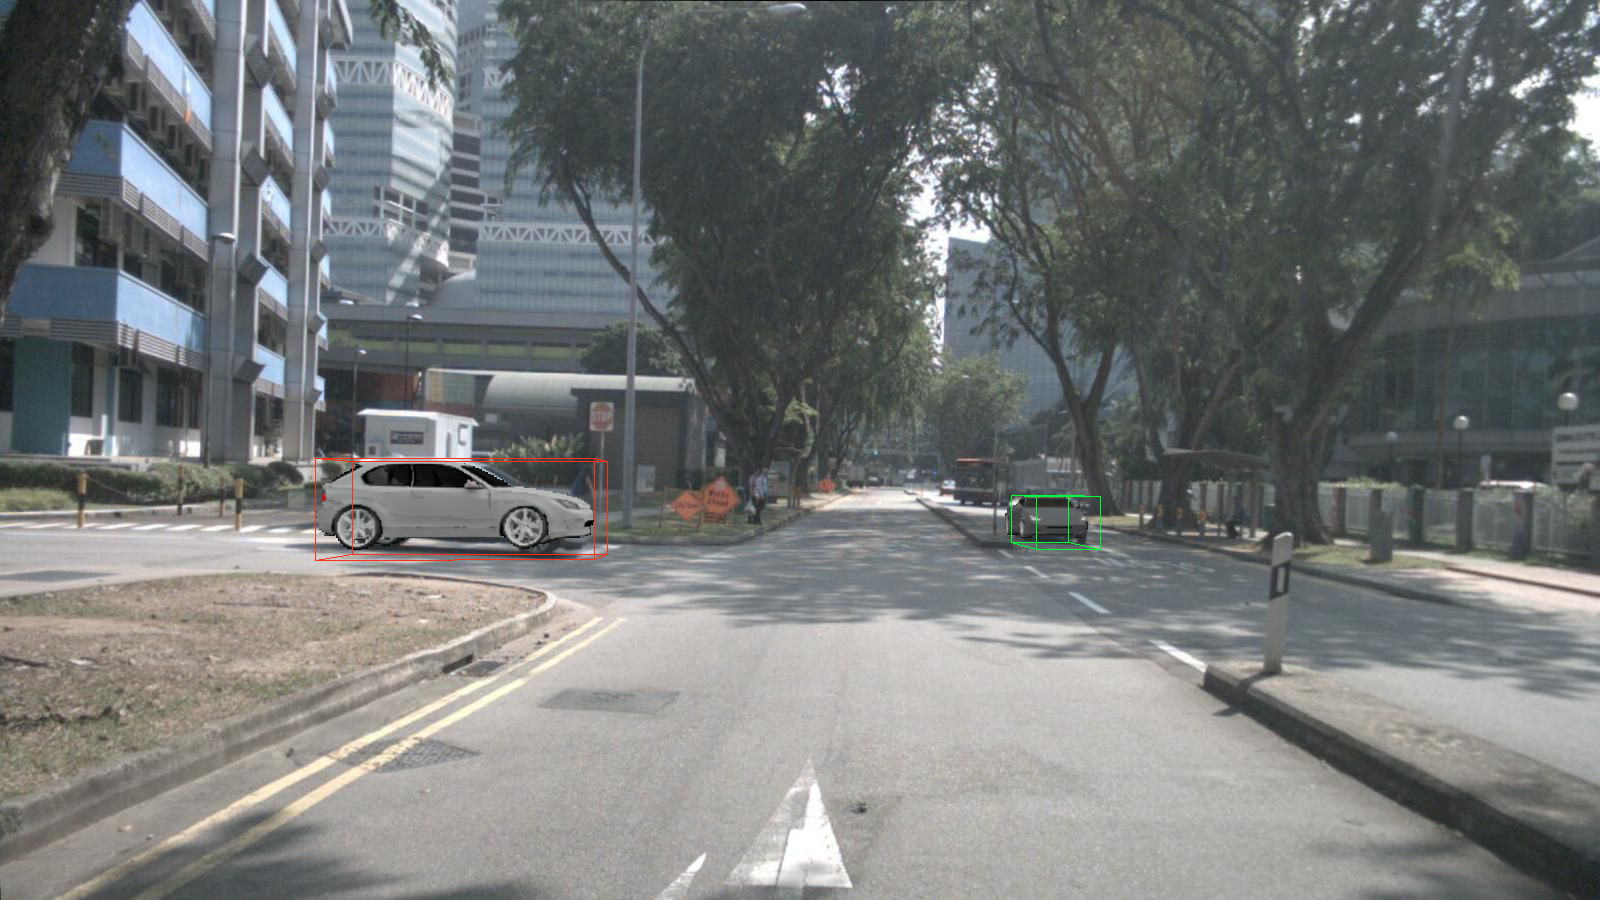
\includegraphics[width=.19\columnwidth, trim={0cm 0cm 0cm 0cm},clip]{fig/nuScenes_main/scene6/35_28_bbox.png}}&
% 		\raisebox{-0.5\height}{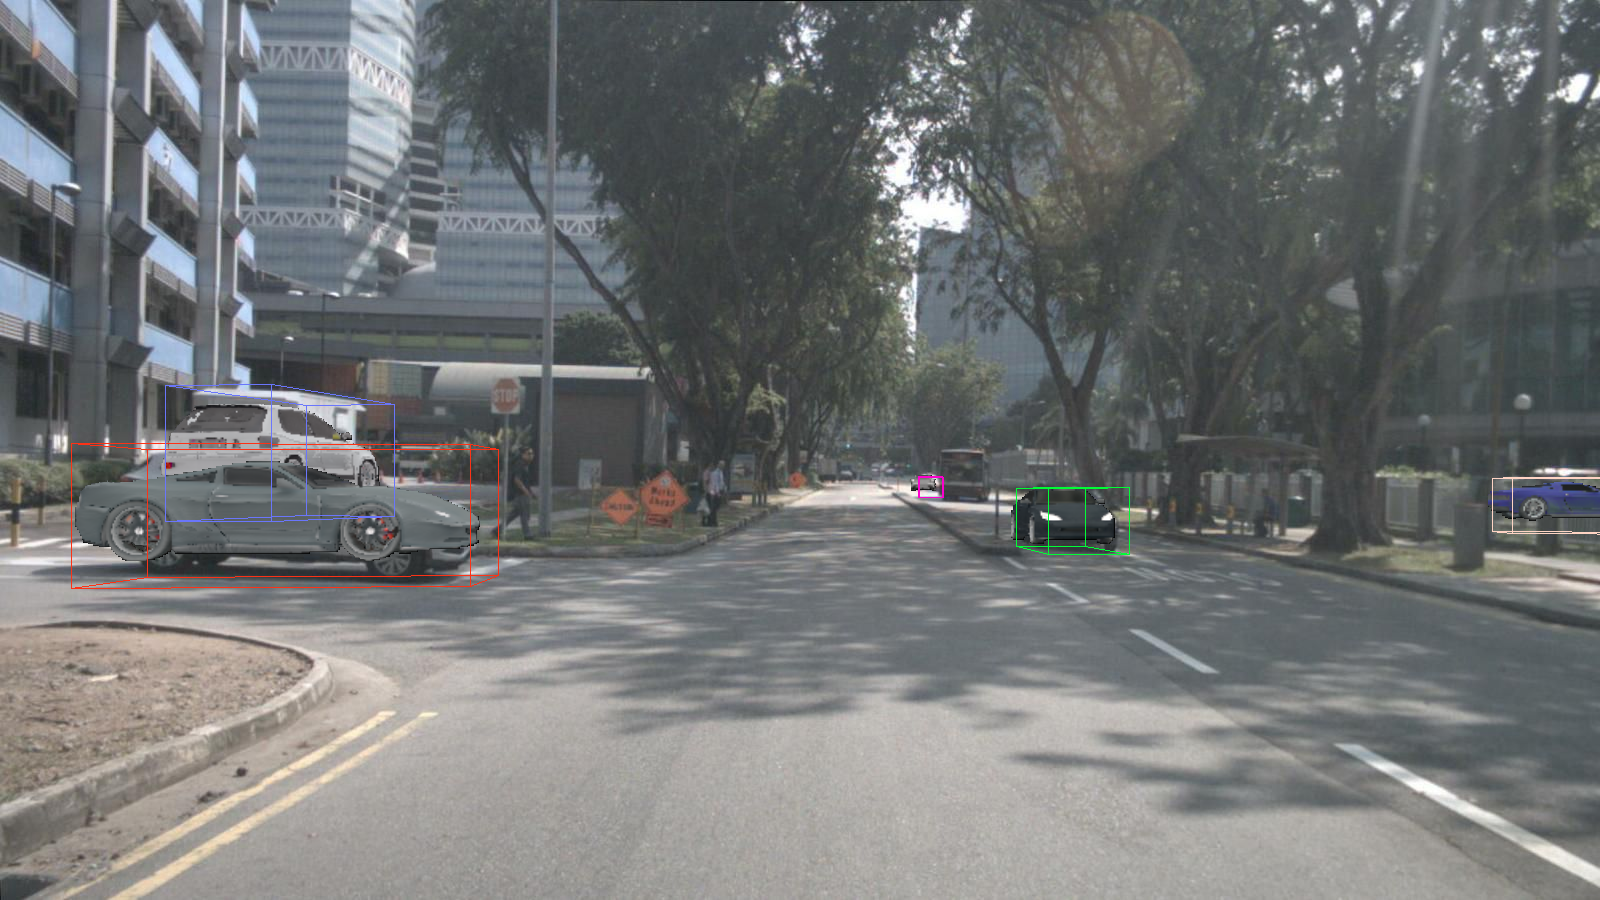
\includegraphics[width=.19\columnwidth, trim={0cm 0cm 0cm 0cm},clip]{fig/nuScenes_main/scene6/35_29_bbox.png}}&
% 		\raisebox{-0.5\height}{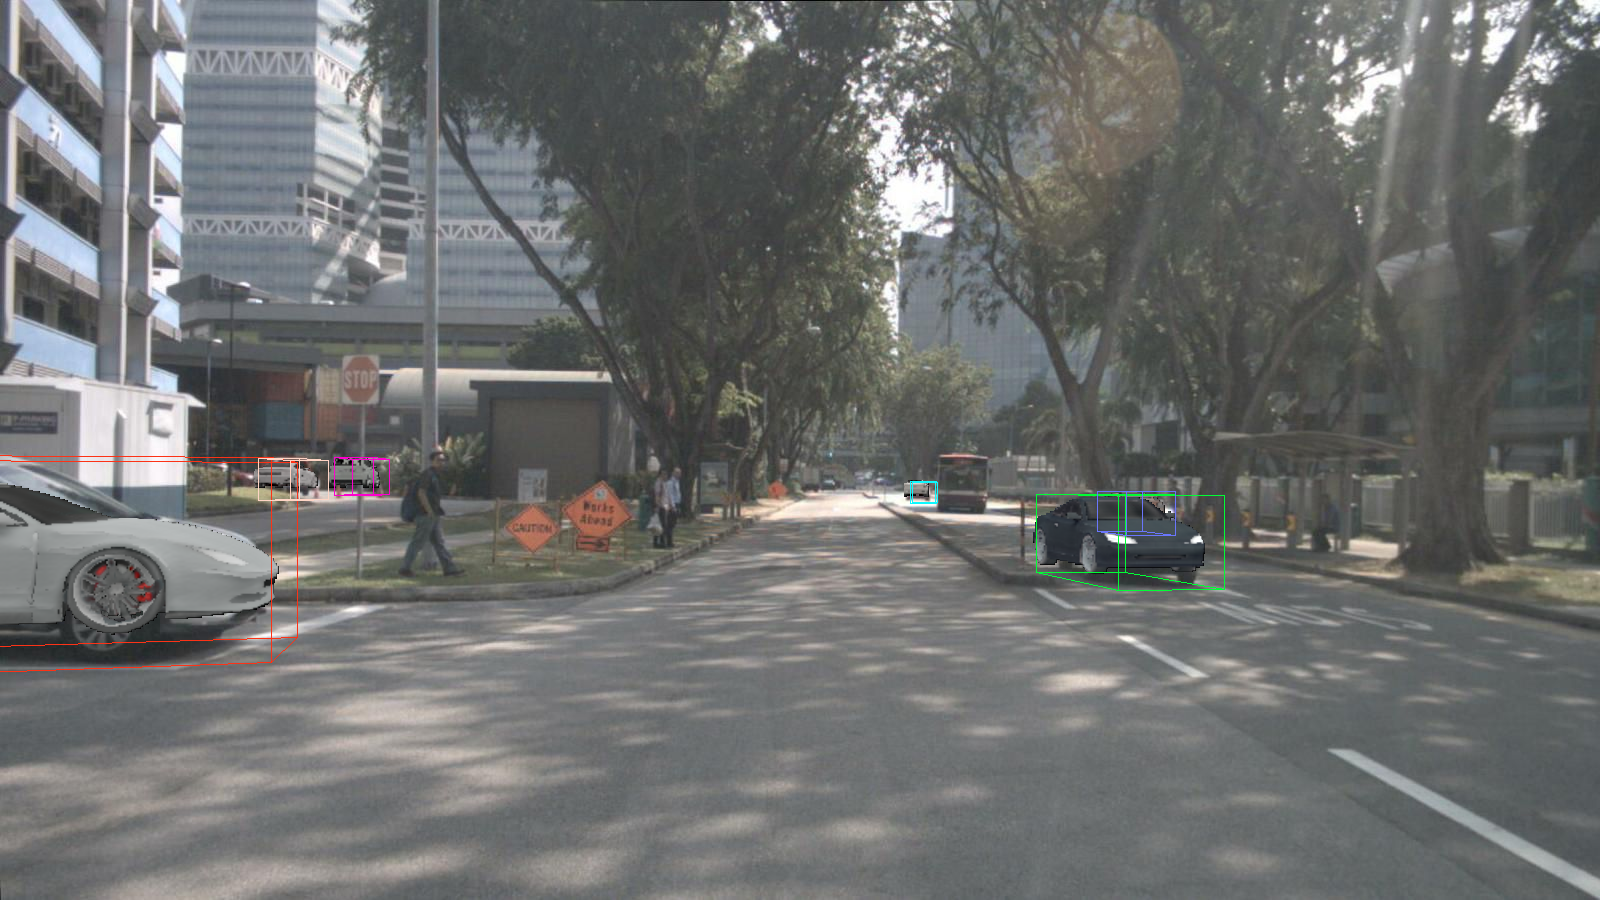
\includegraphics[width=.19\columnwidth, trim={0cm 0cm 0cm 0cm},clip]{fig/nuScenes_main/scene6/35_30_bbox.png}}&
% 		\raisebox{-0.5\height}{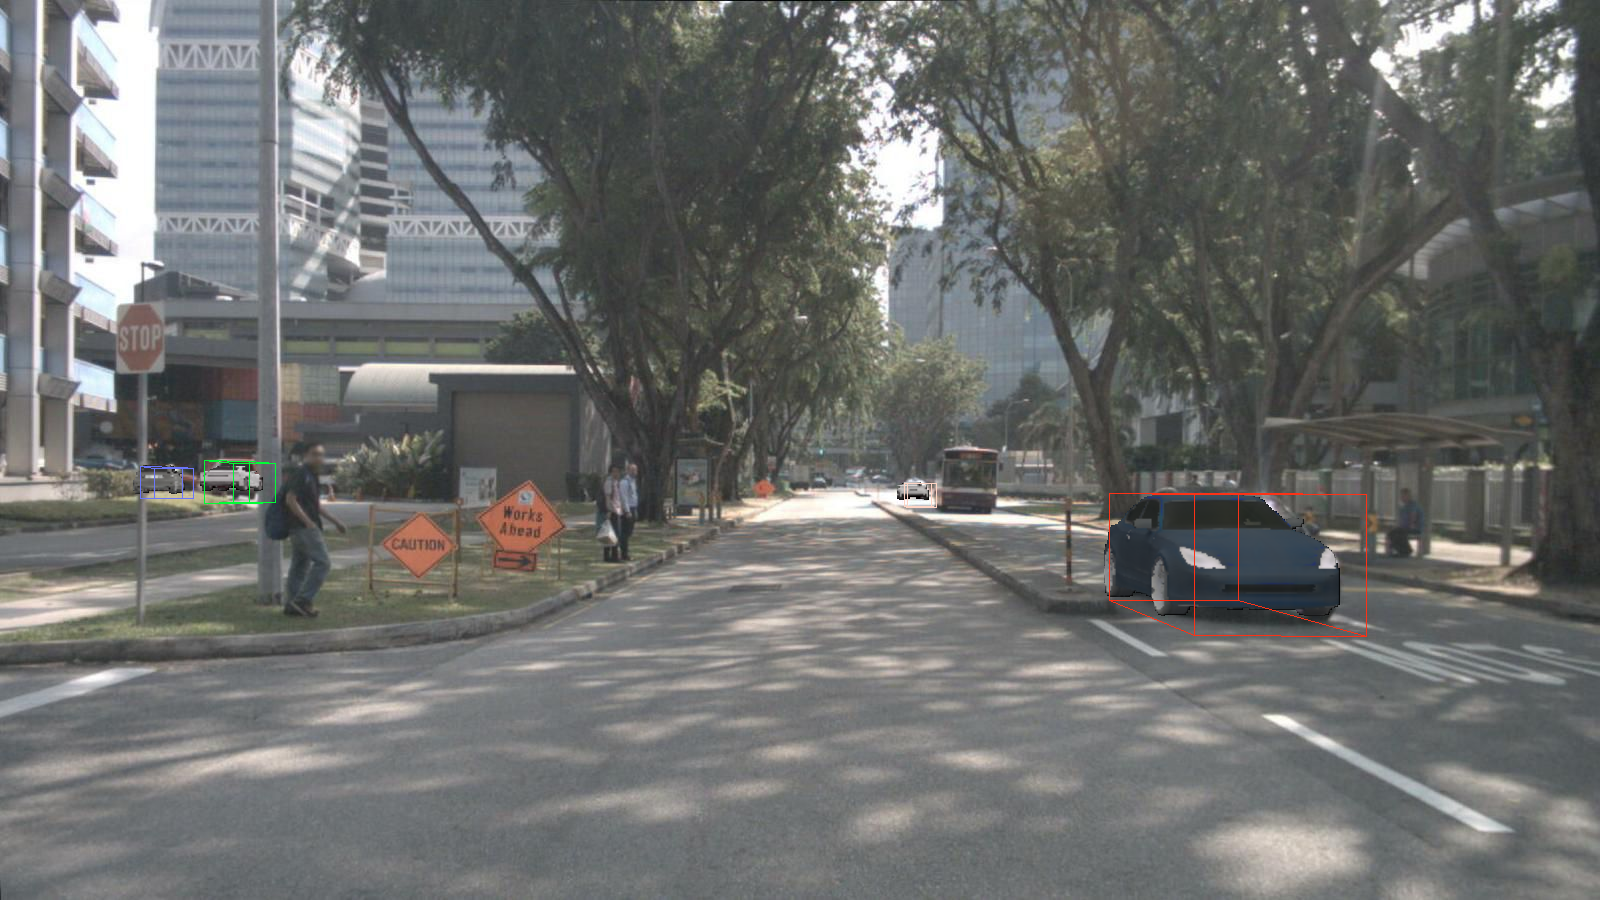
\includegraphics[width=.19\columnwidth, trim={0cm 0cm 0cm 0cm},clip]{fig/nuScenes_main/scene6/35_31_bbox.png}}\\[0.7cm]
  
%             \rotatebox[origin=c]{90}{{\footnotesize	Parking lot}}&
%   		\raisebox{-0.5\height}{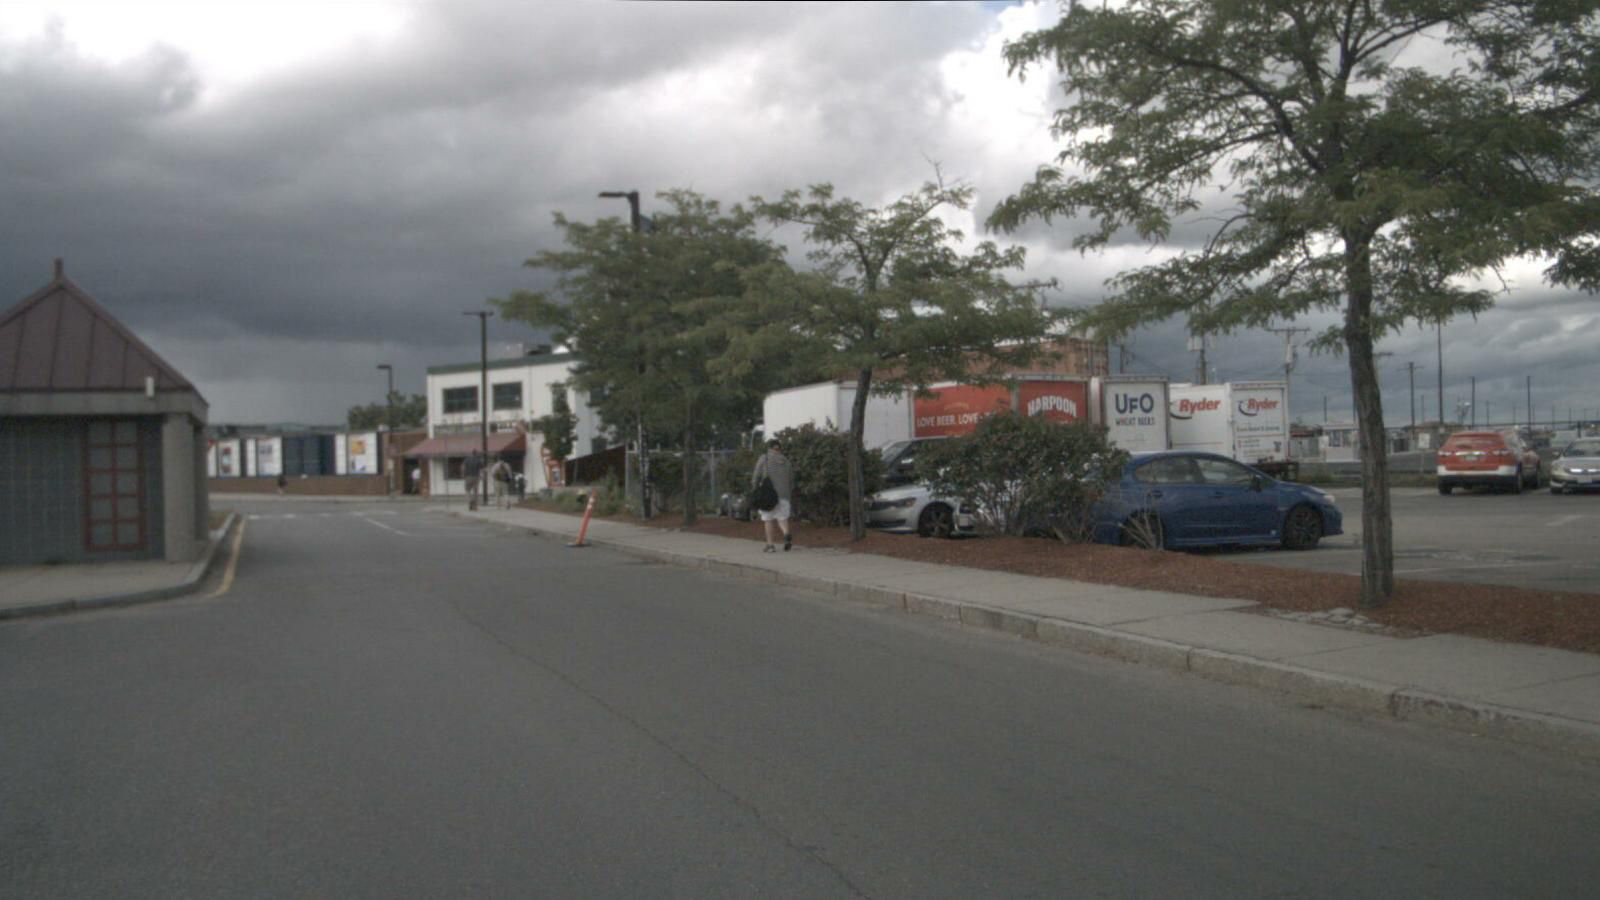
\includegraphics[width=.19\columnwidth, trim={0cm 0cm 0cm 0cm},clip]{fig/nuScenes_main/scene7/gt_2.png}}&
% 		\raisebox{-0.5\height}{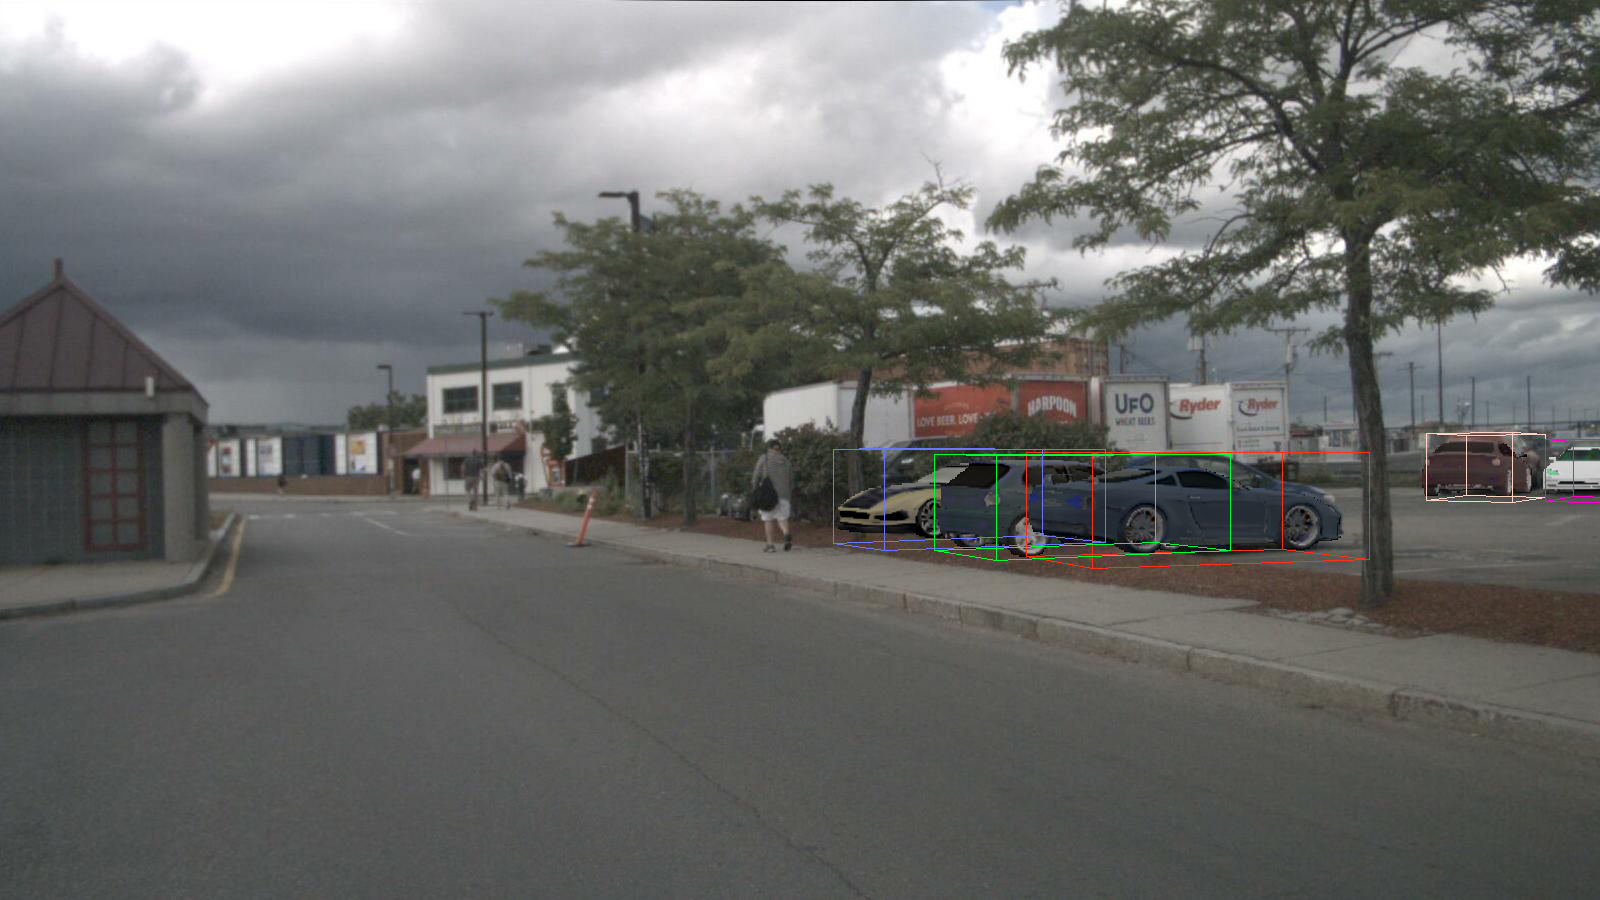
\includegraphics[width=.19\columnwidth, trim={0cm 0cm 0cm 0cm},clip]{fig/nuScenes_main/scene7/bbox_0.png}}&
% 		\raisebox{-0.5\height}{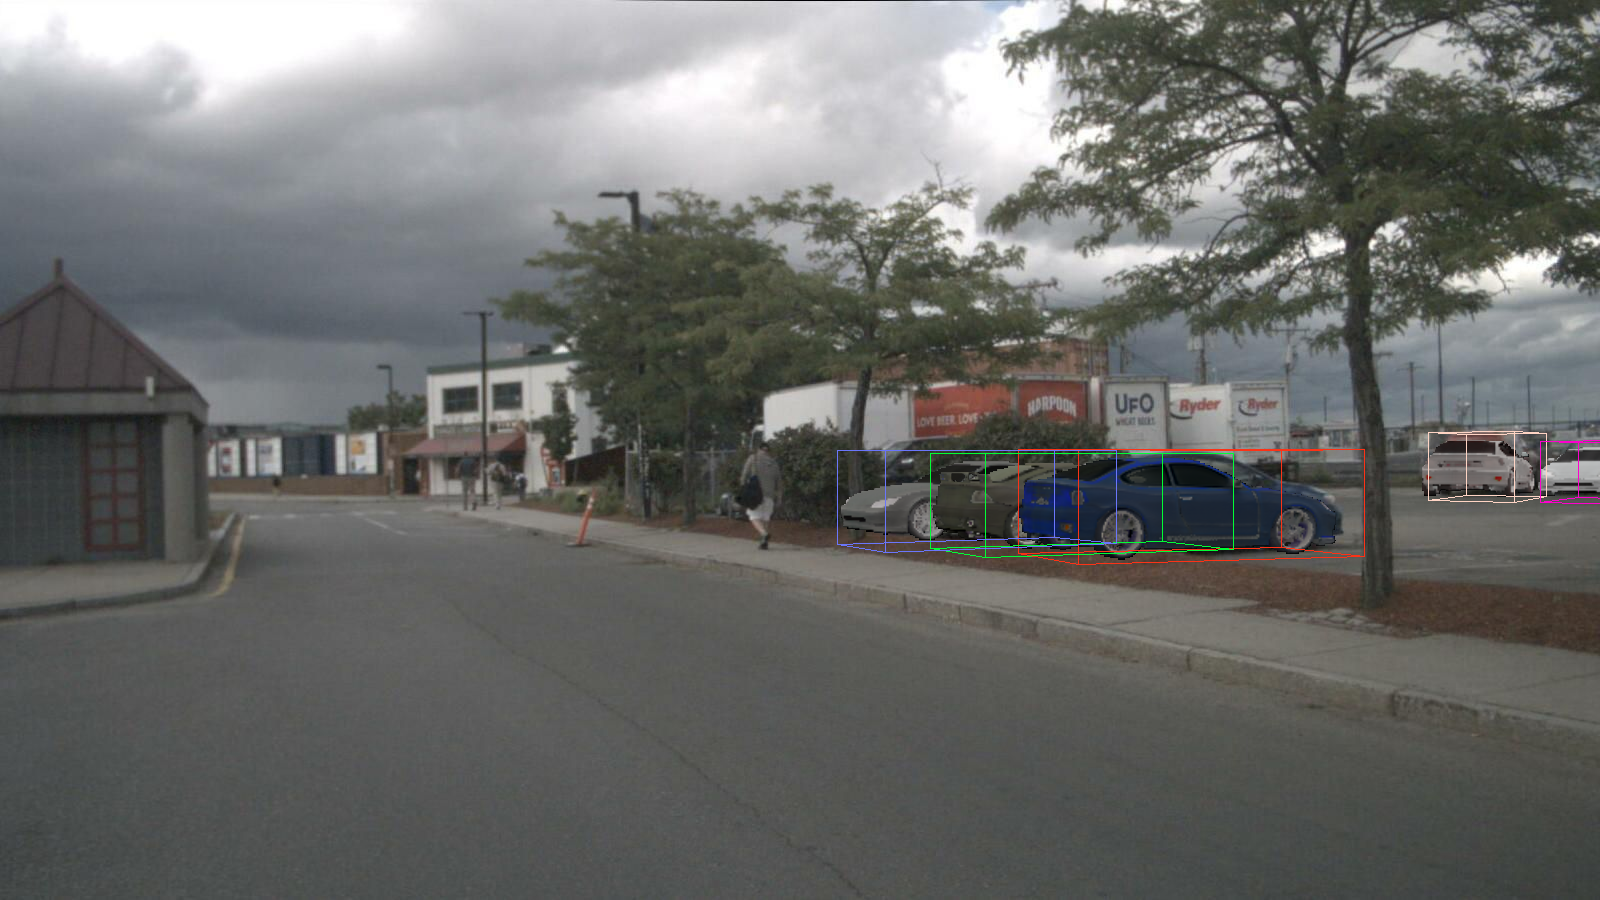
\includegraphics[width=.19\columnwidth, trim={0cm 0cm 0cm 0cm},clip]{fig/nuScenes_main/scene7/bbox_1.png}}&
% 		\raisebox{-0.5\height}{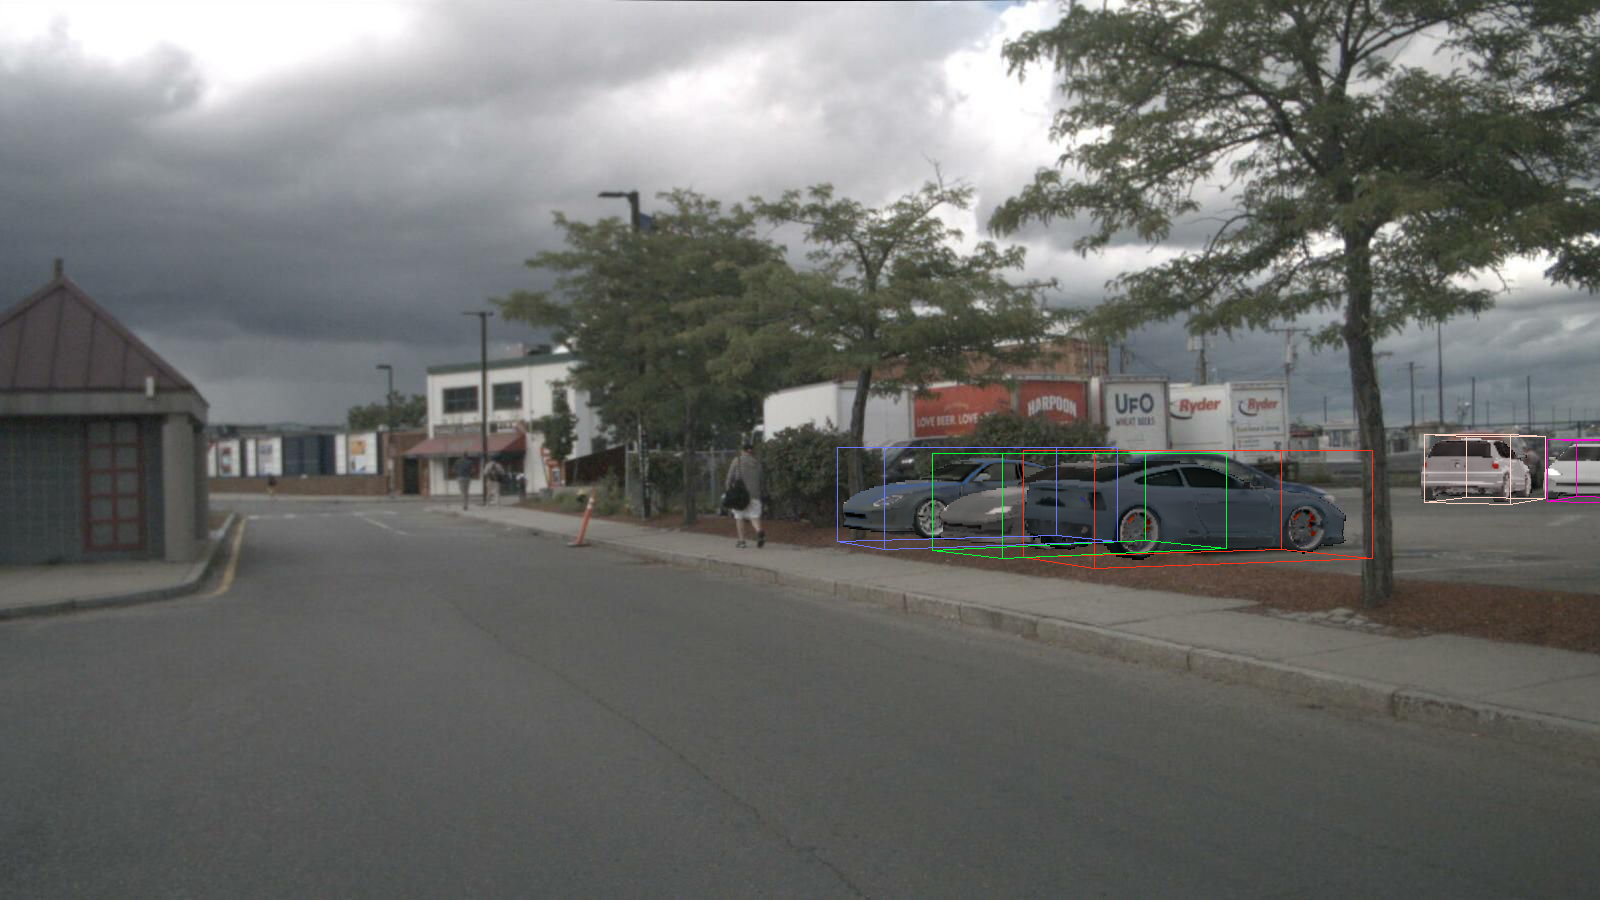
\includegraphics[width=.19\columnwidth, trim={0cm 0cm 0cm 0cm},clip]{fig/nuScenes_main/scene7/bbox_3.png}}&
% 		\raisebox{-0.5\height}{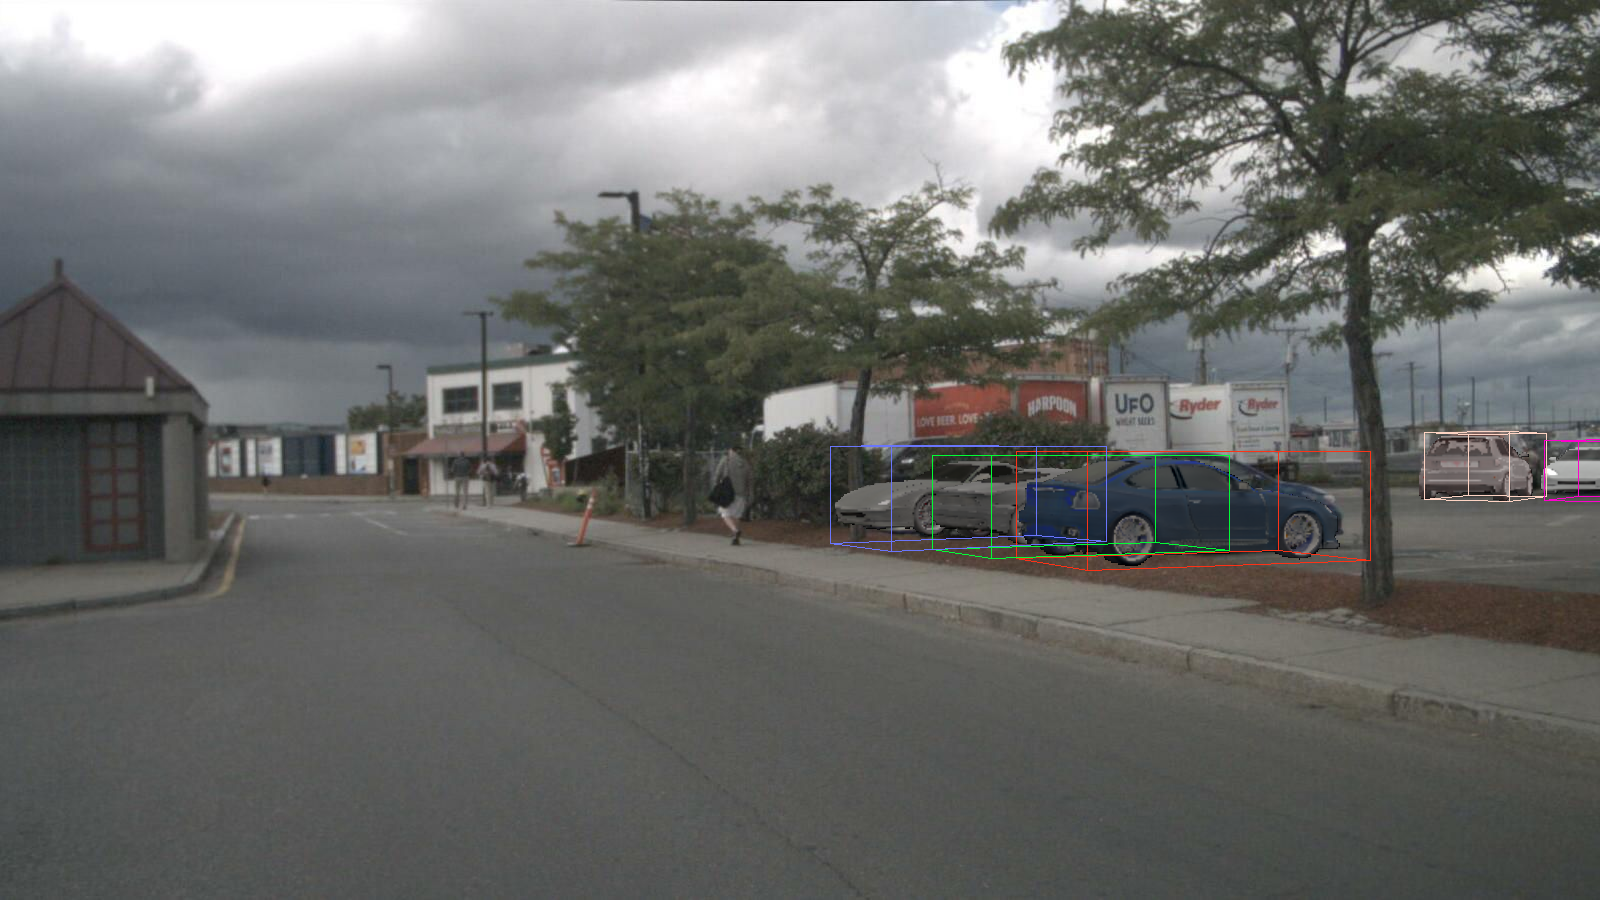
\includegraphics[width=.19\columnwidth, trim={0cm 0cm 0cm 0cm},clip]{fig/nuScenes_main/scene7/bbox_33.png}}\\%[0.95cm]
		
% 	\end{tabular}
% }
% 	\vspace{-6pt}
% 	\caption{Tracking via Inverse Neural Rendering on nuScenes~\cite{caesar2020nuscenes}. From left to right, we show (i) observed images from diverse scenes at timestep $k=0$; (ii) an overlay of the optimized generated object and its 3D bounding boxes at timestep $k=0, 1, 2 \text{ and } 3$. The color of the bounding boxes for each object corresponds to the predicted tracklet ID. We see that even in such diverse scenarios, our method does not lose any tracks and performs robustly across all scenarios, although the dataset is unseen.}
% 	\label{fig:nuScenes_results}
%  	\vspace{-12pt}
% \end{figure*}

\begin{figure*}[t!]
	% \vspace{-20pt}
	\centering
	\resizebox{1.\linewidth}{!}{
	\renewcommand{\arraystretch}{0.5}
	\begin{tabular}{@{}c@{\hskip 0.05cm}c@{\hskip 0.05cm}c@{\hskip 0.05cm}c@{\hskip 0.05cm}c@{\hskip 0.05cm}c@{}}
		\centering
            &
		{\small Input $t_0$}&
		{\small Tracked $t_0$}&
		{\small Tracked $t_1$}&
		{\small Tracked $t_2$}&
		{\small Tracked $t_3$}\\

            \rotatebox[origin=c]{90}{{\footnotesize	  Suburban}}&
		 \raisebox{-0.5\height}{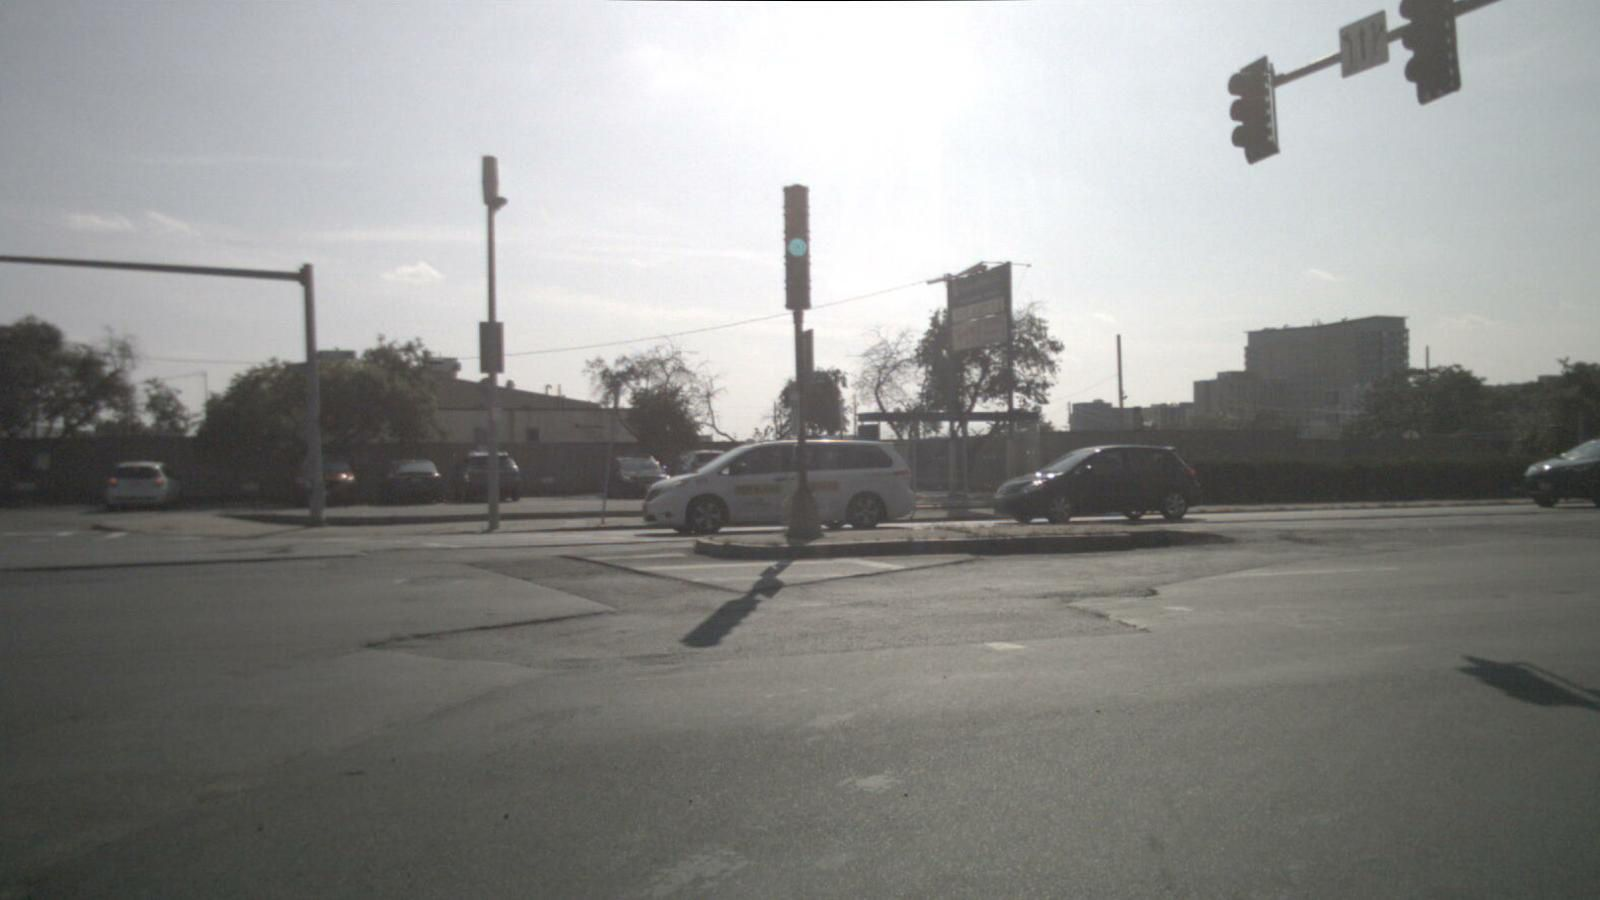
\includegraphics[width=.32\columnwidth, trim={0cm 0cm 0cm 0cm},clip]{fig/nuScenes_main/scene2/0484_2_gt.png}}&
		 \raisebox{-0.5\height}{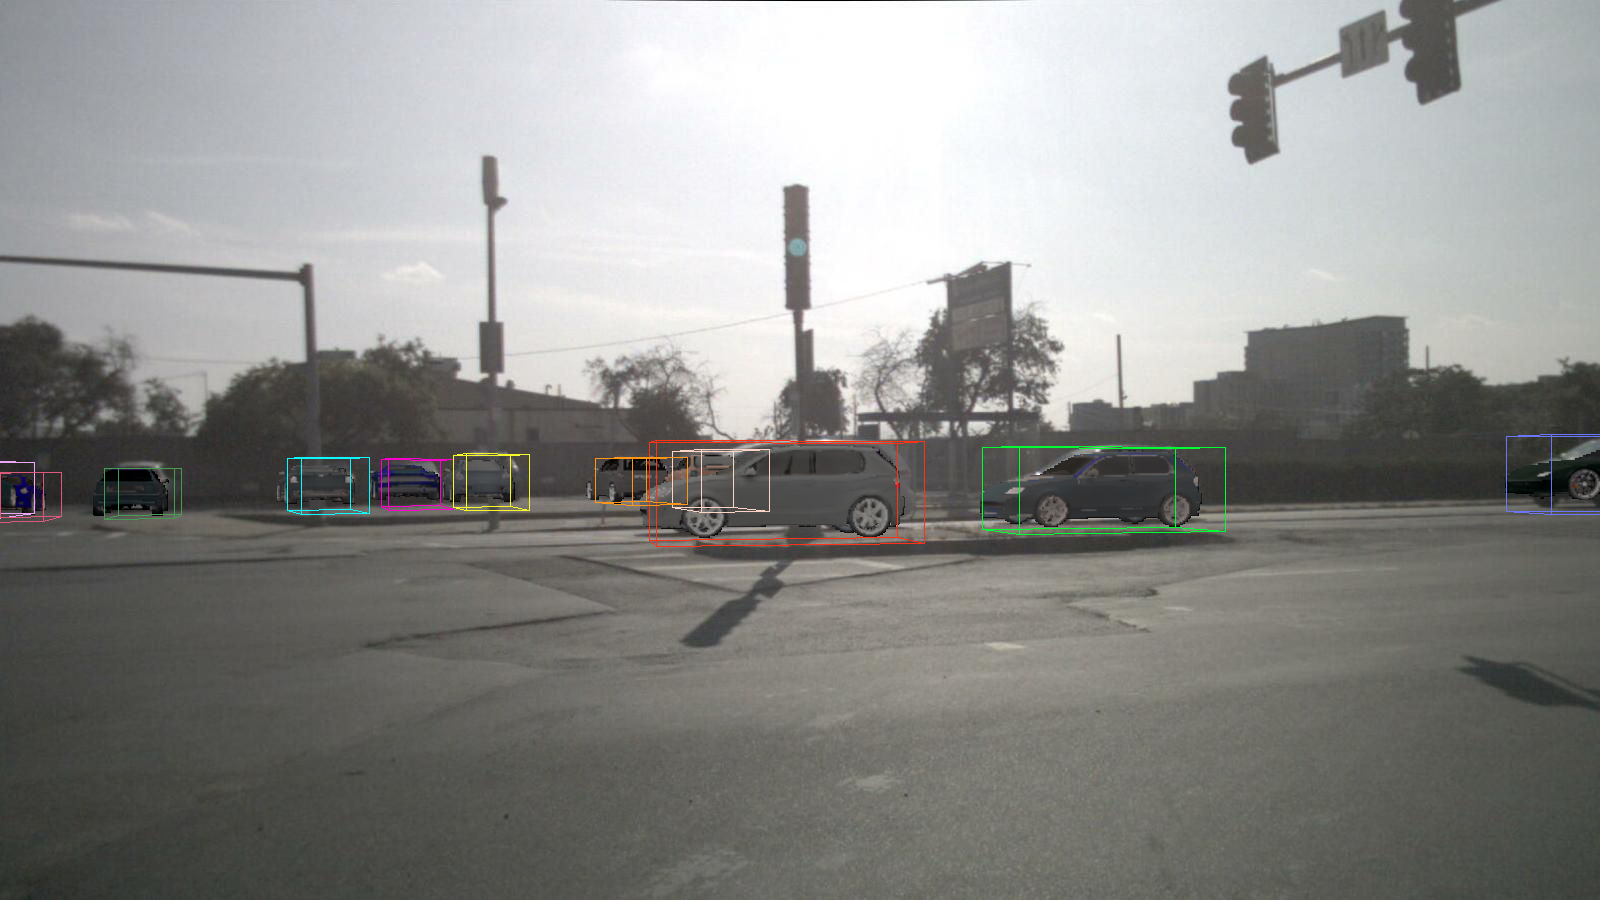
\includegraphics[width=.32\columnwidth, trim={0cm 0cm 0cm 0cm},clip]{fig/nuScenes_main/scene2/0484_2_bbox.png}}&
		 \raisebox{-0.5\height}{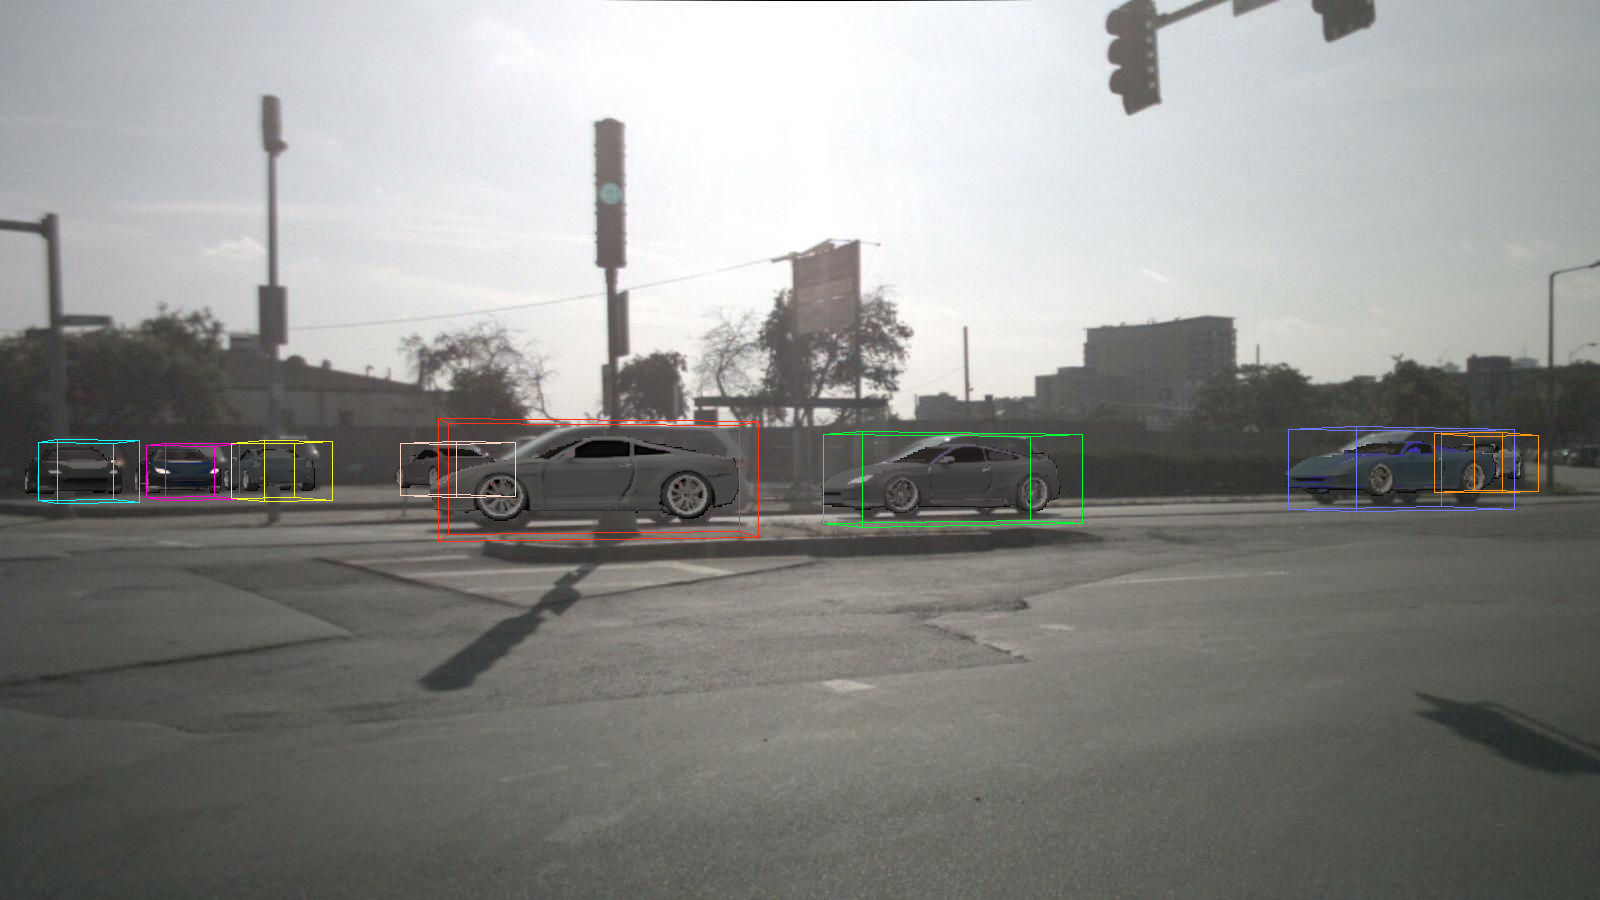
\includegraphics[width=.32\columnwidth, trim={0cm 0cm 0cm 0cm},clip]{fig/nuScenes_main/scene2/0484_3_bbox.png}}&
		 \raisebox{-0.5\height}{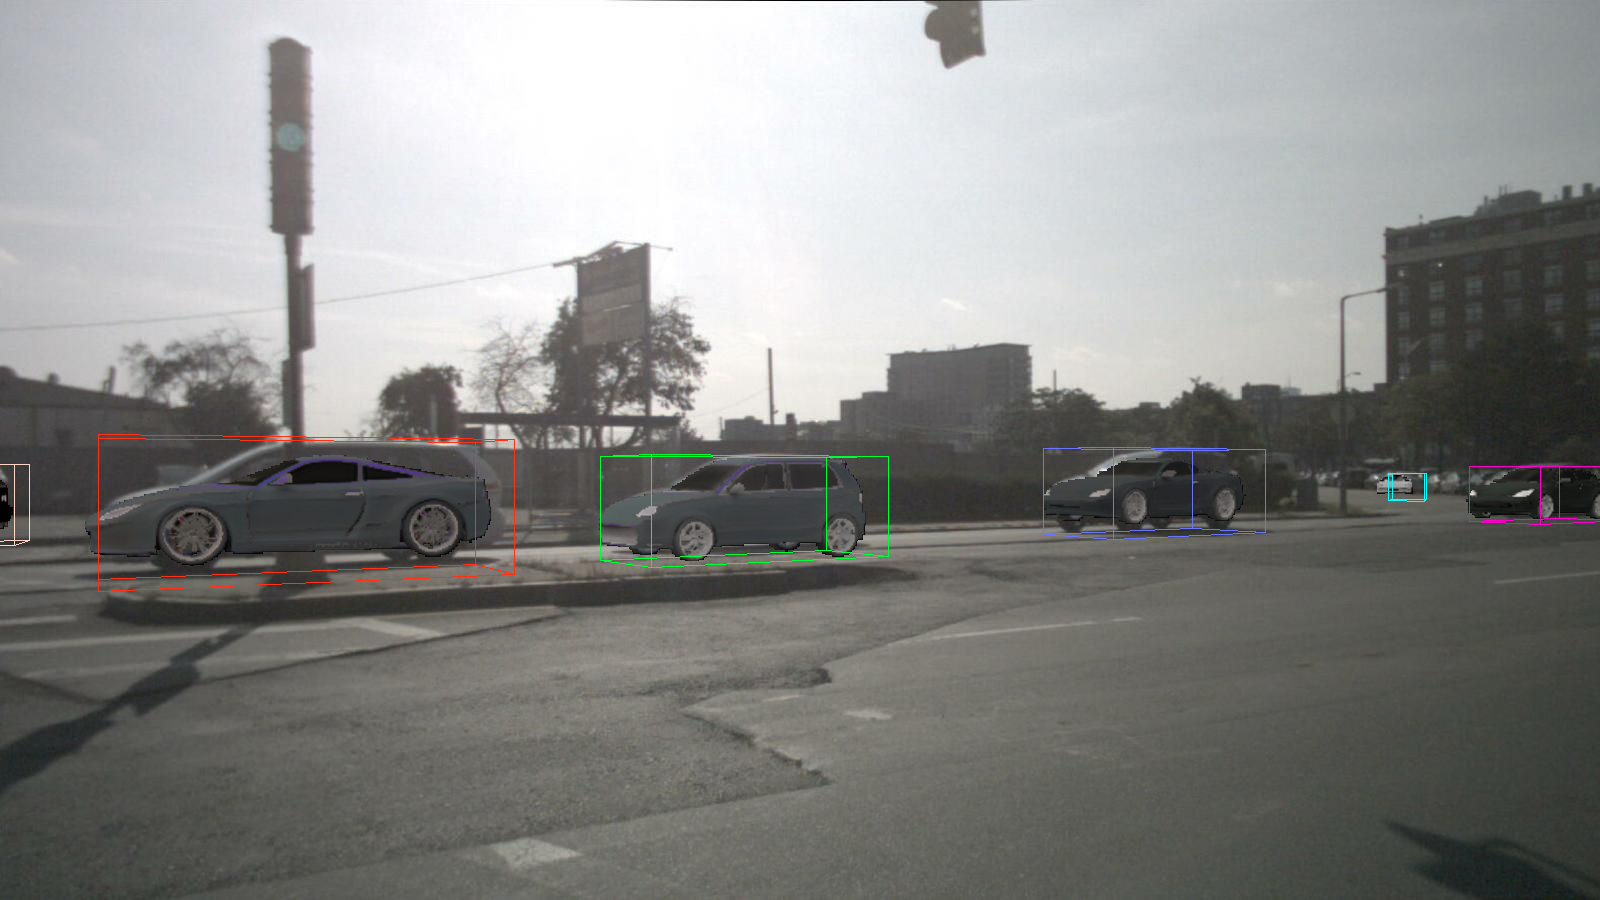
\includegraphics[width=.32\columnwidth, trim={0cm 0cm 0cm 0cm},clip]{fig/nuScenes_main/scene2/0484_4_bbox.png}}&
		 \raisebox{-0.5\height}{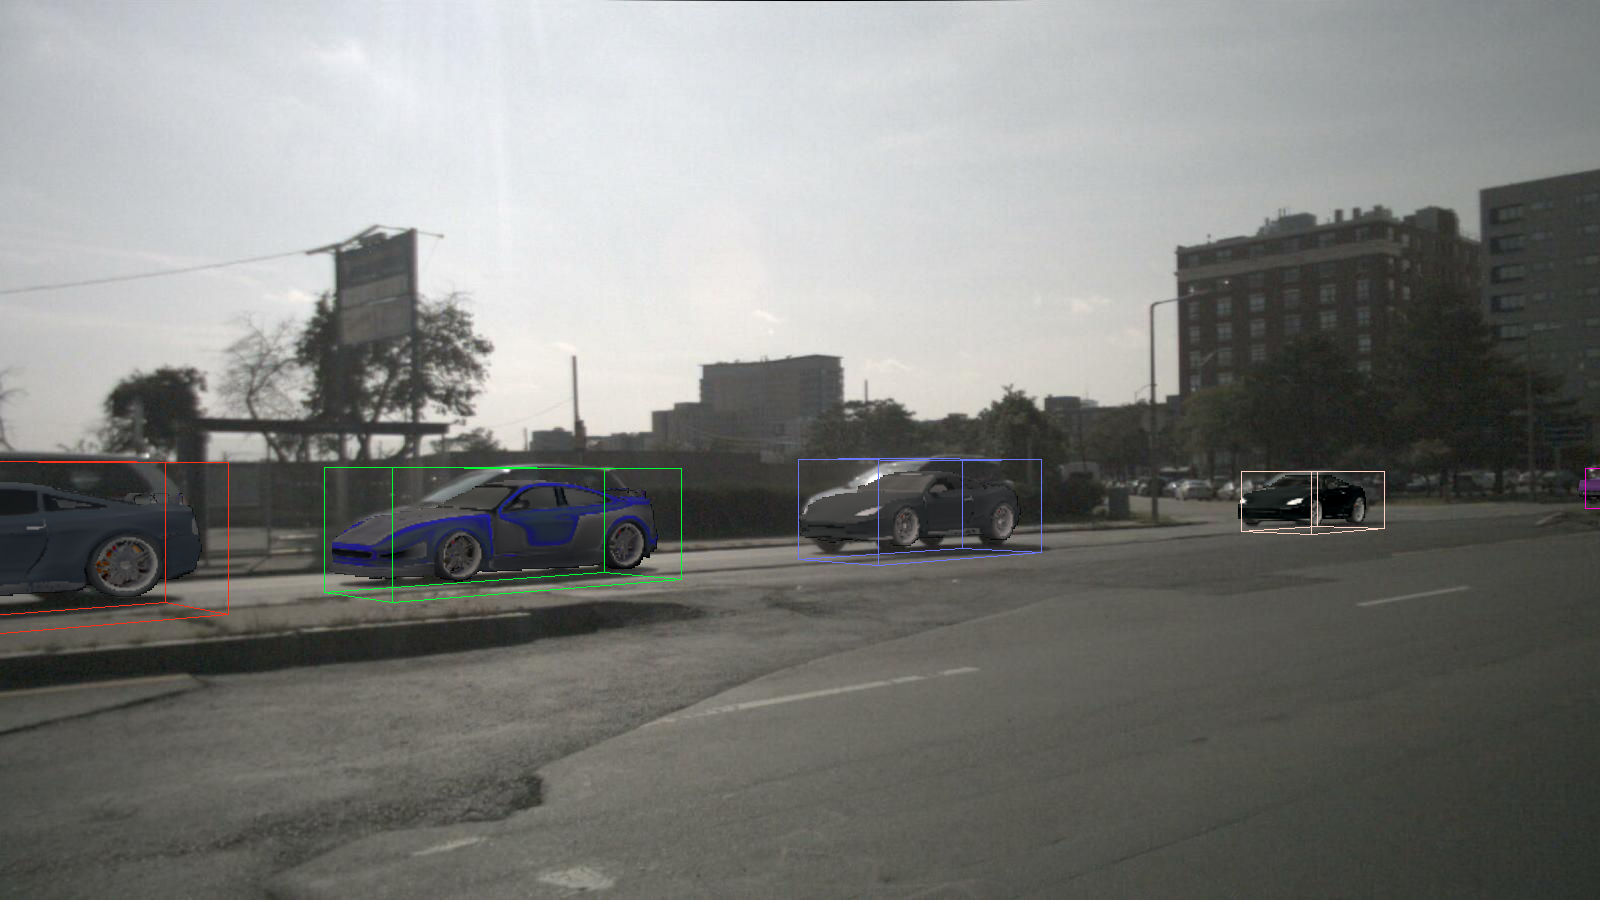
\includegraphics[width=.32\columnwidth, trim={0cm 0cm 0cm 0cm},clip]{fig/nuScenes_main/scene2/0484_5_bbox.png}}\\[1.1cm]
  
		\rotatebox[origin=c]{90}{{\footnotesize	 Dense Urban}}&
		\raisebox{-0.5\height}{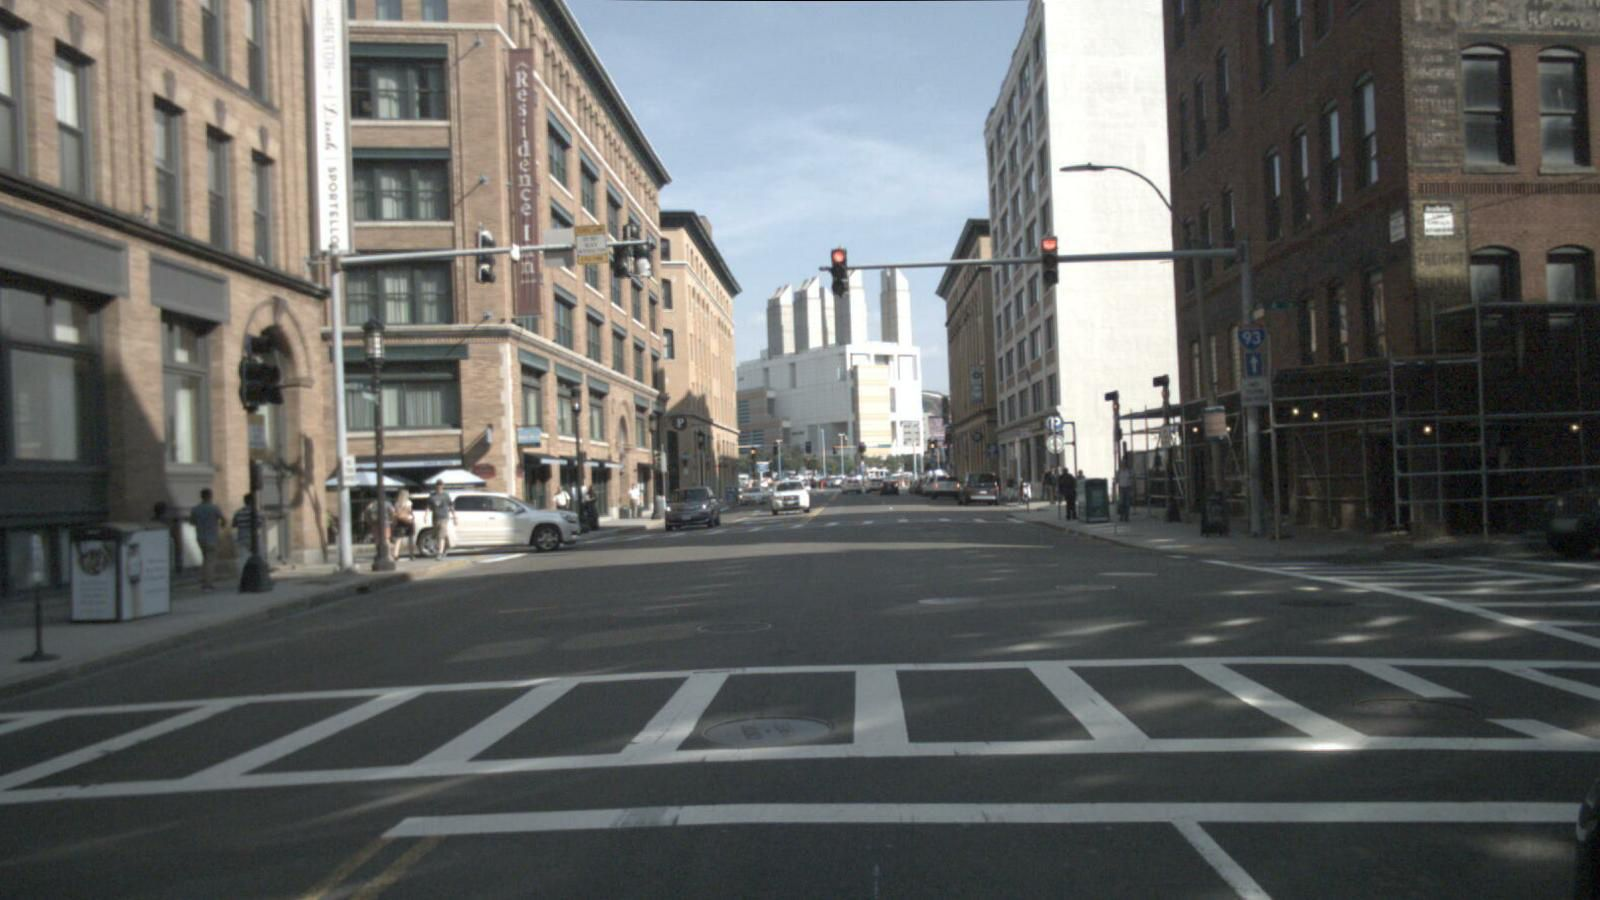
\includegraphics[width=.32\columnwidth, trim={0cm 0cm 0cm 0cm},clip]{fig/nuScenes_main/scene3/0496_30_gt.png}}&
		\raisebox{-0.5\height}{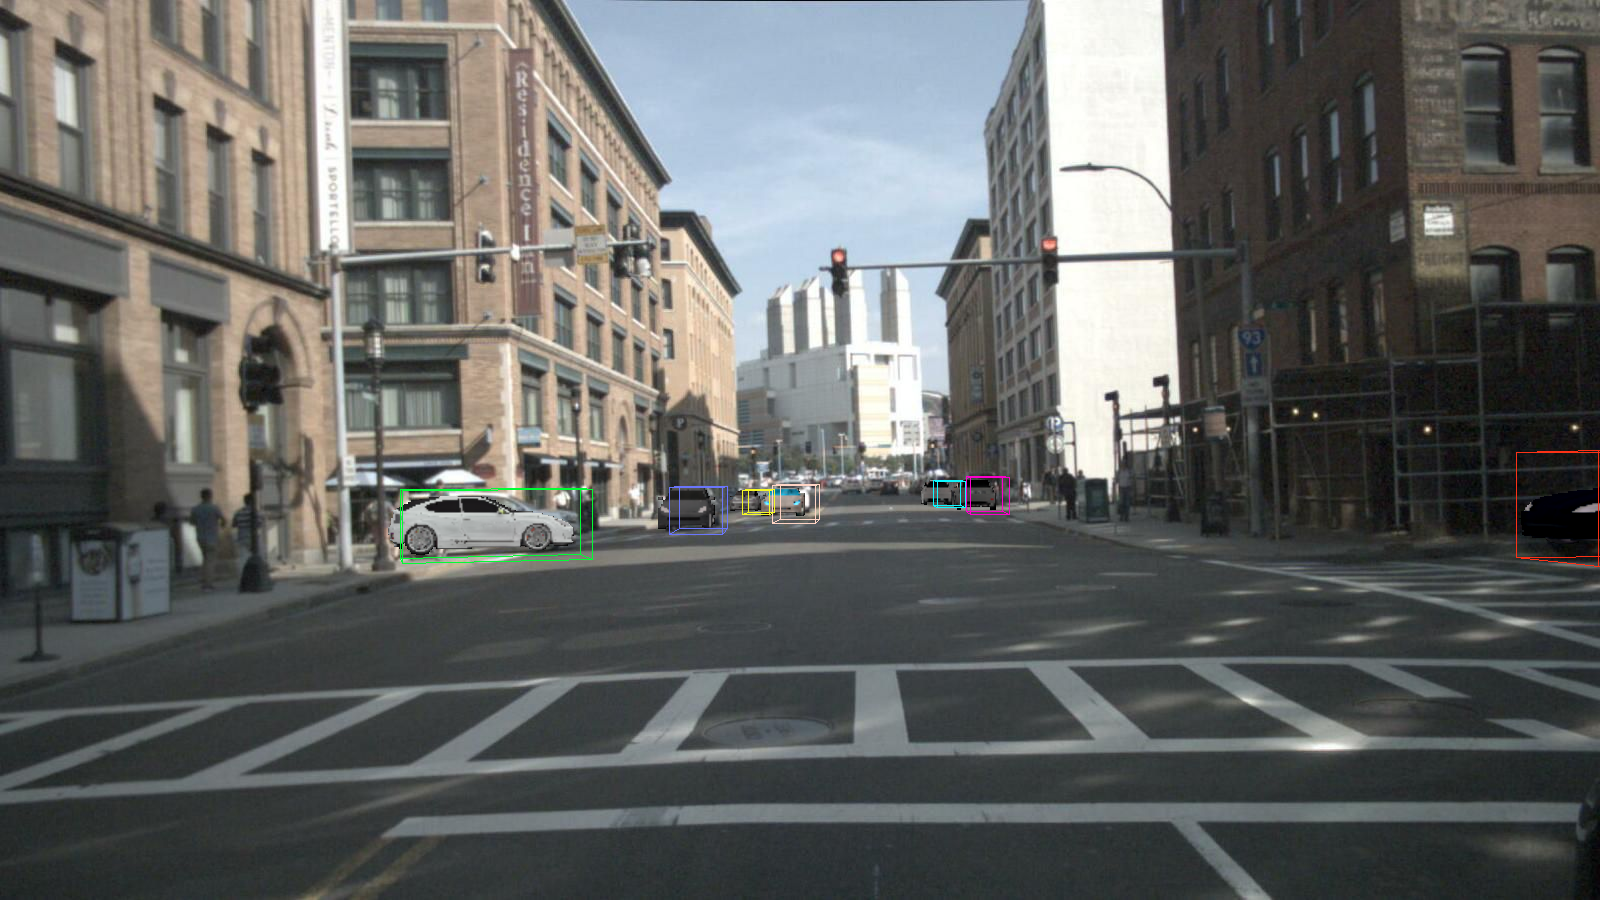
\includegraphics[width=.32\columnwidth, trim={0cm 0cm 0cm 0cm},clip]{fig/nuScenes_main/scene3/0496_30_bbox.png}} &
		\raisebox{-0.5\height}{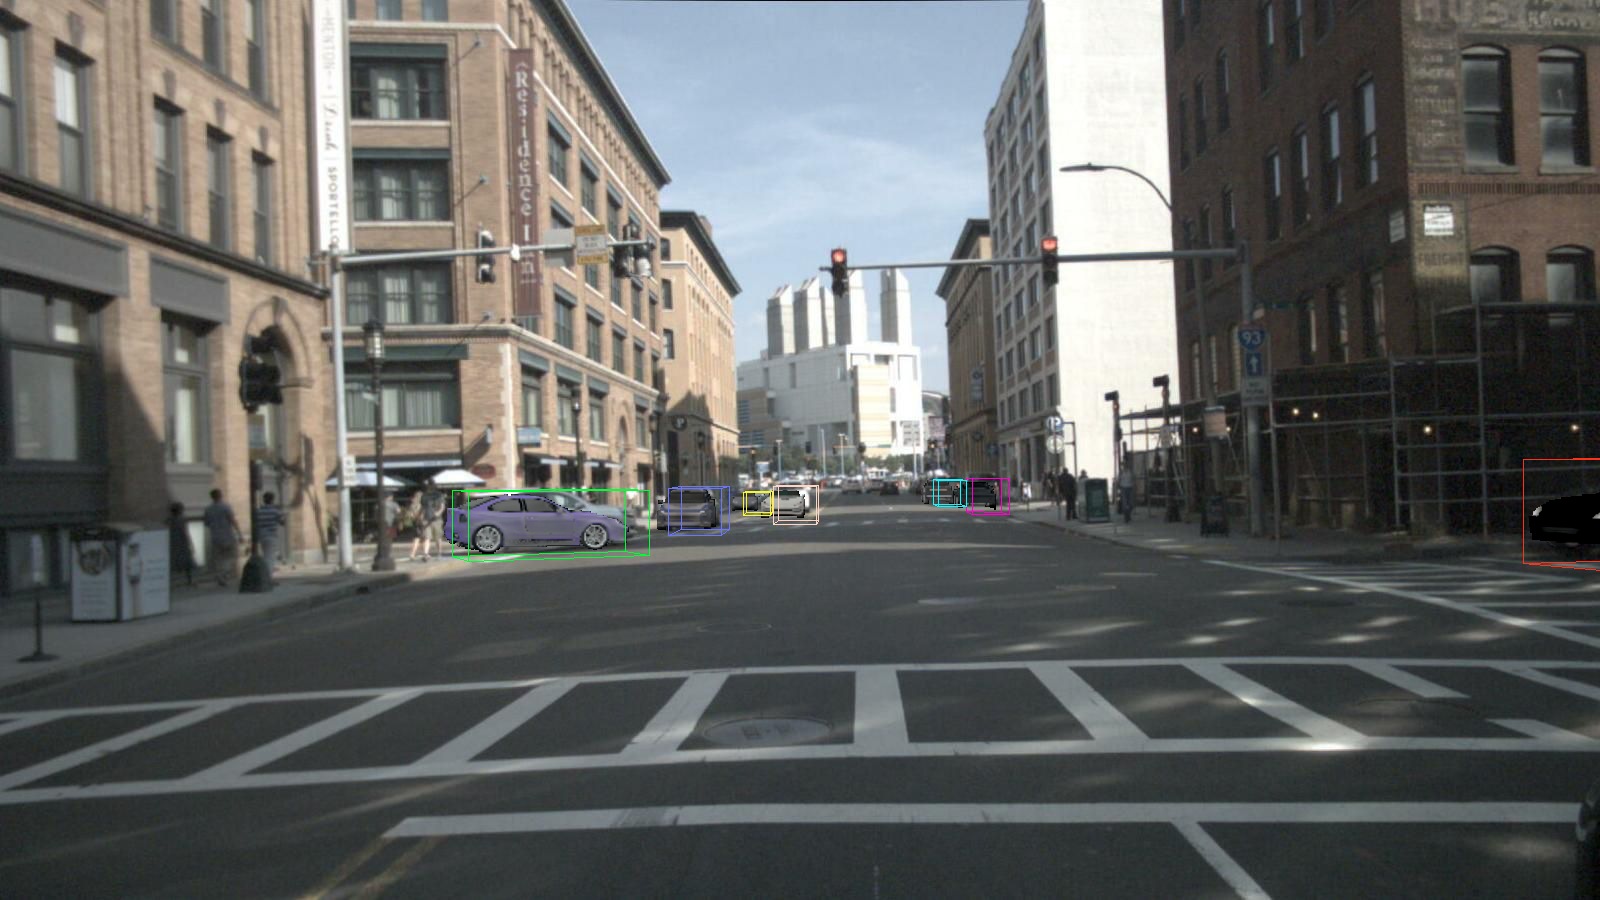
\includegraphics[width=.32\columnwidth, trim={0cm 0cm 0cm 0cm},clip]{fig/nuScenes_main/scene3/0496_31_bbox.png}}&
		\raisebox{-0.5\height}{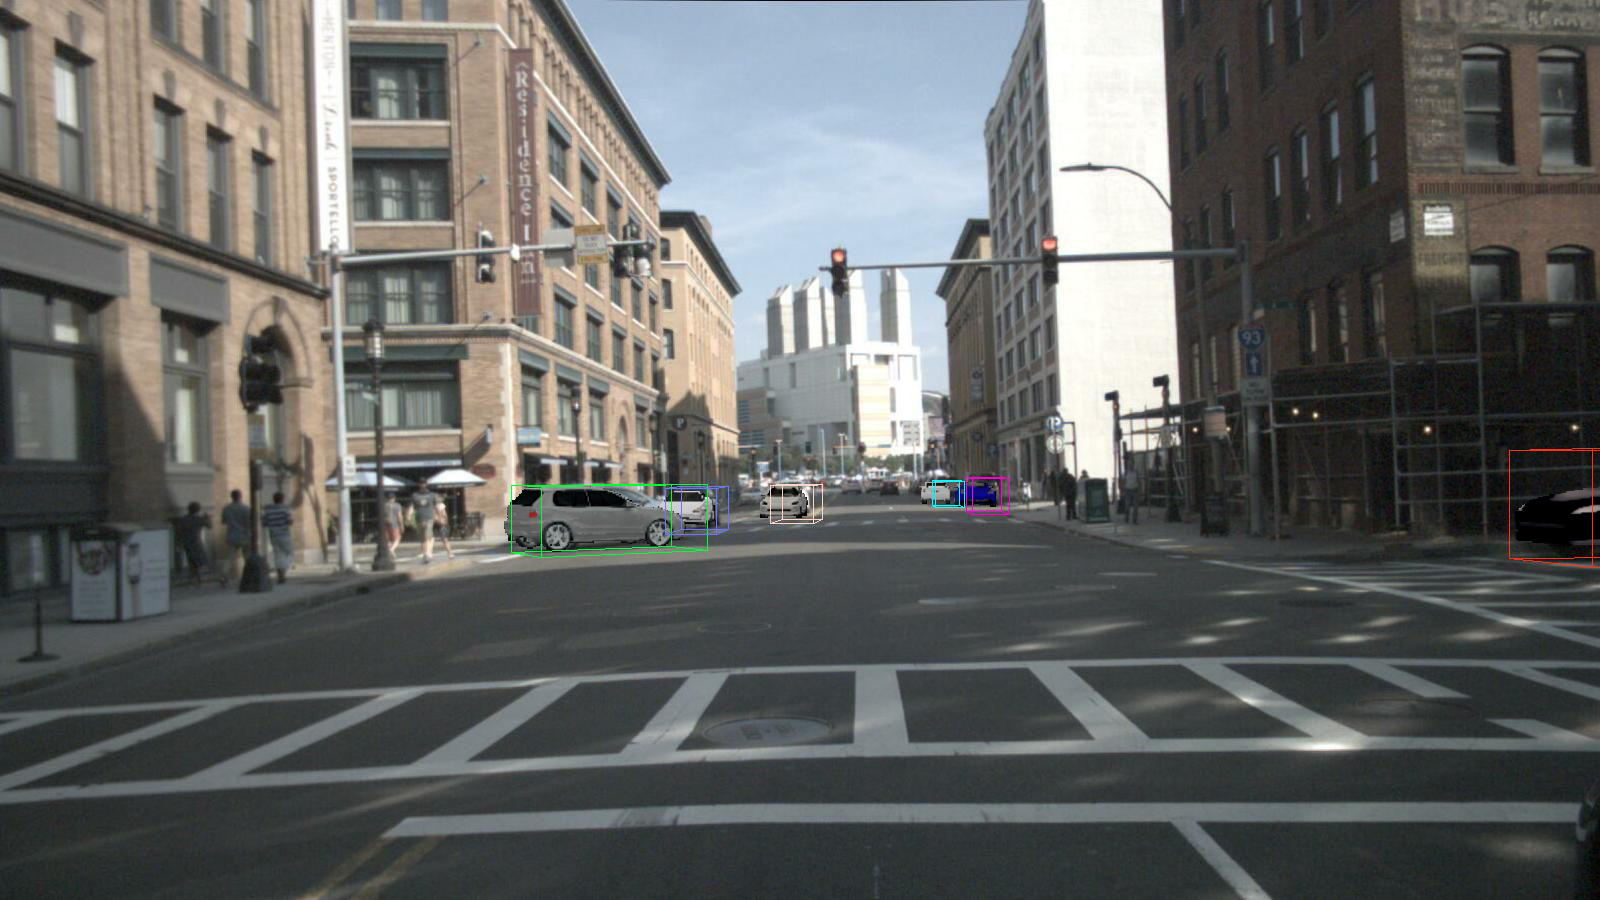
\includegraphics[width=.32\columnwidth, trim={0cm 0cm 0cm 0cm},clip]{fig/nuScenes_main/scene3/0496_32_bbox.png}}&
		\raisebox{-0.5\height}{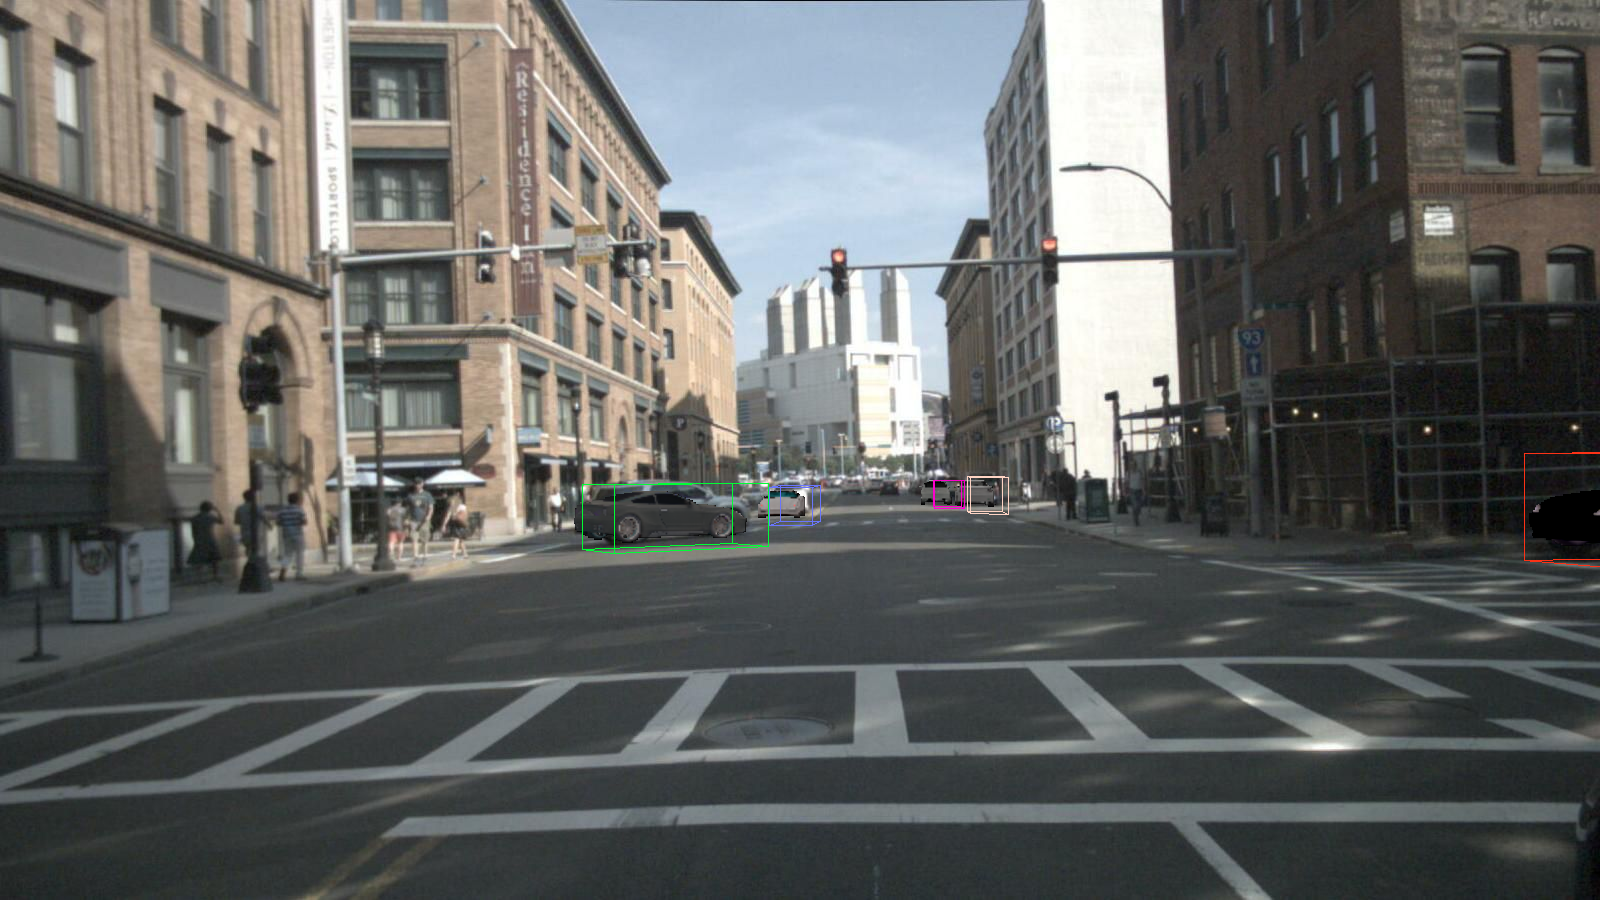
\includegraphics[width=.32\columnwidth, trim={0cm 0cm 0cm 0cm},clip]{fig/nuScenes_main/scene3/0496_33_bbox.png}}\\[1.1cm]
  
            \rotatebox[origin=c]{90}{{\footnotesize	 Clutter}}&
  		\raisebox{-0.5\height}{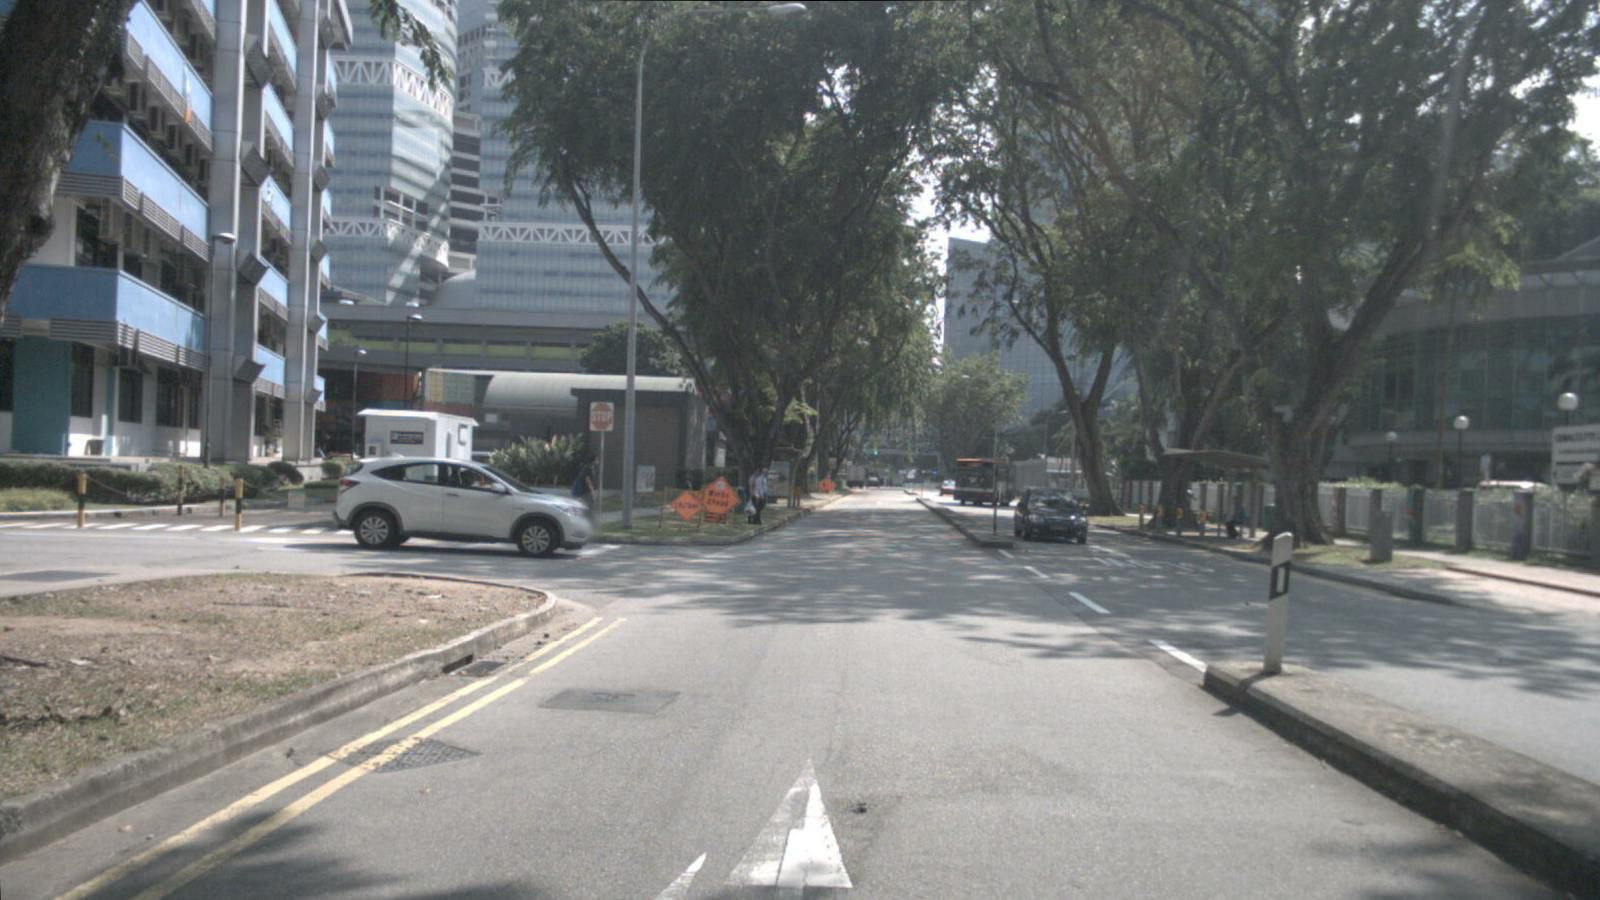
\includegraphics[width=.32\columnwidth, trim={0cm 0cm 0cm 0cm},clip]{fig/nuScenes_main/scene6/28_gt_img.png}}&
		\raisebox{-0.5\height}{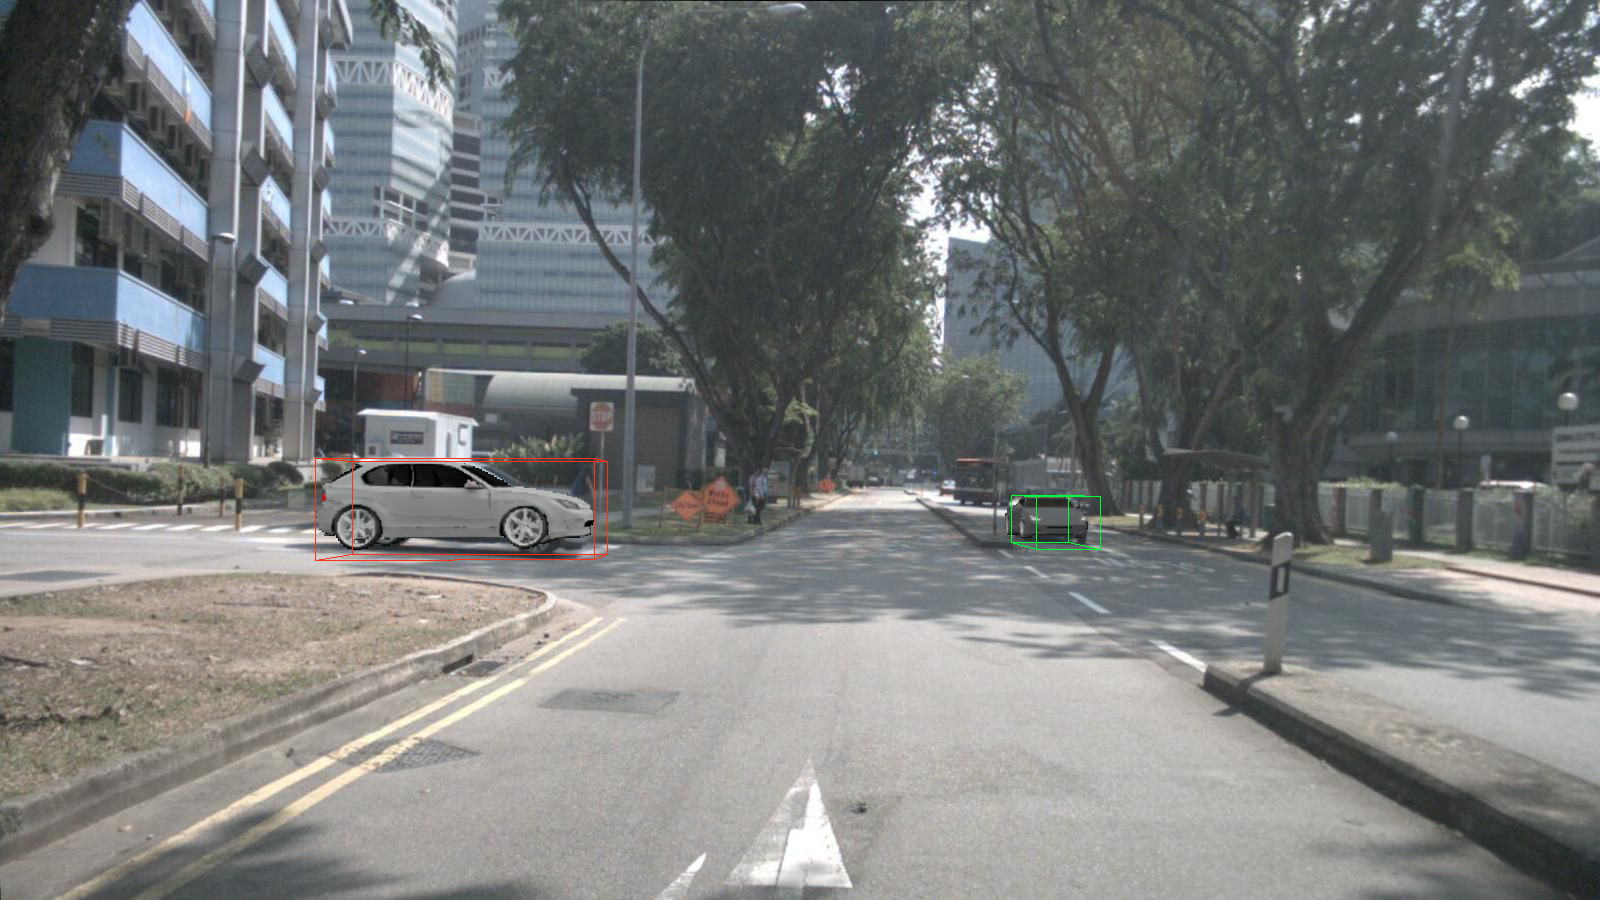
\includegraphics[width=.32\columnwidth, trim={0cm 0cm 0cm 0cm},clip]{fig/nuScenes_main/scene6/35_28_bbox.png}}&
		\raisebox{-0.5\height}{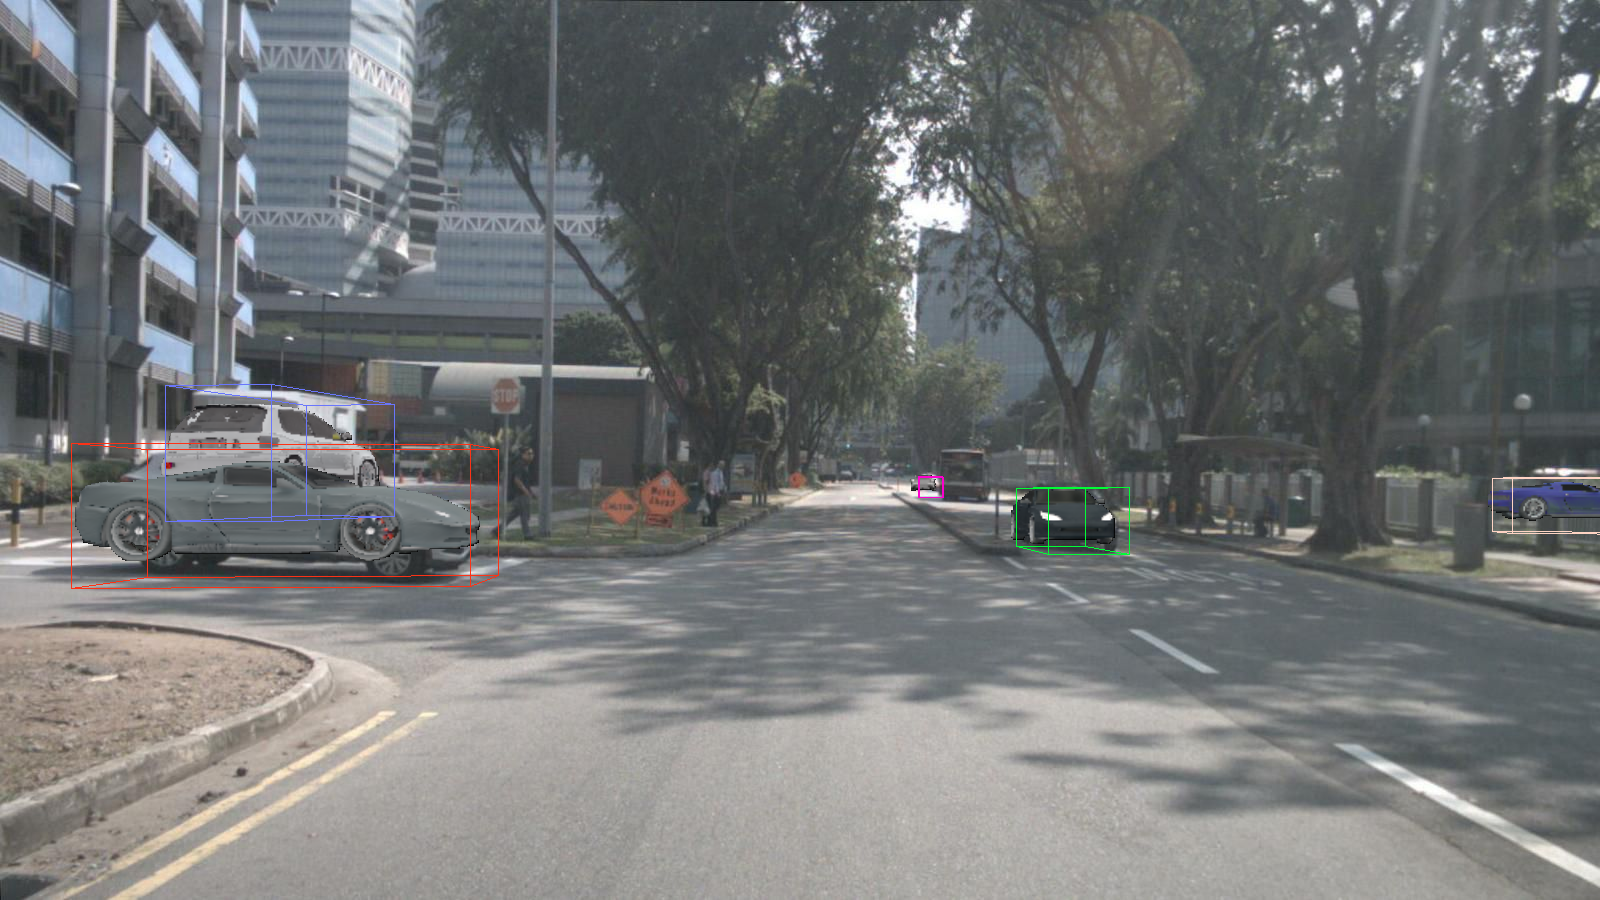
\includegraphics[width=.32\columnwidth, trim={0cm 0cm 0cm 0cm},clip]{fig/nuScenes_main/scene6/35_29_bbox.png}}&
		\raisebox{-0.5\height}{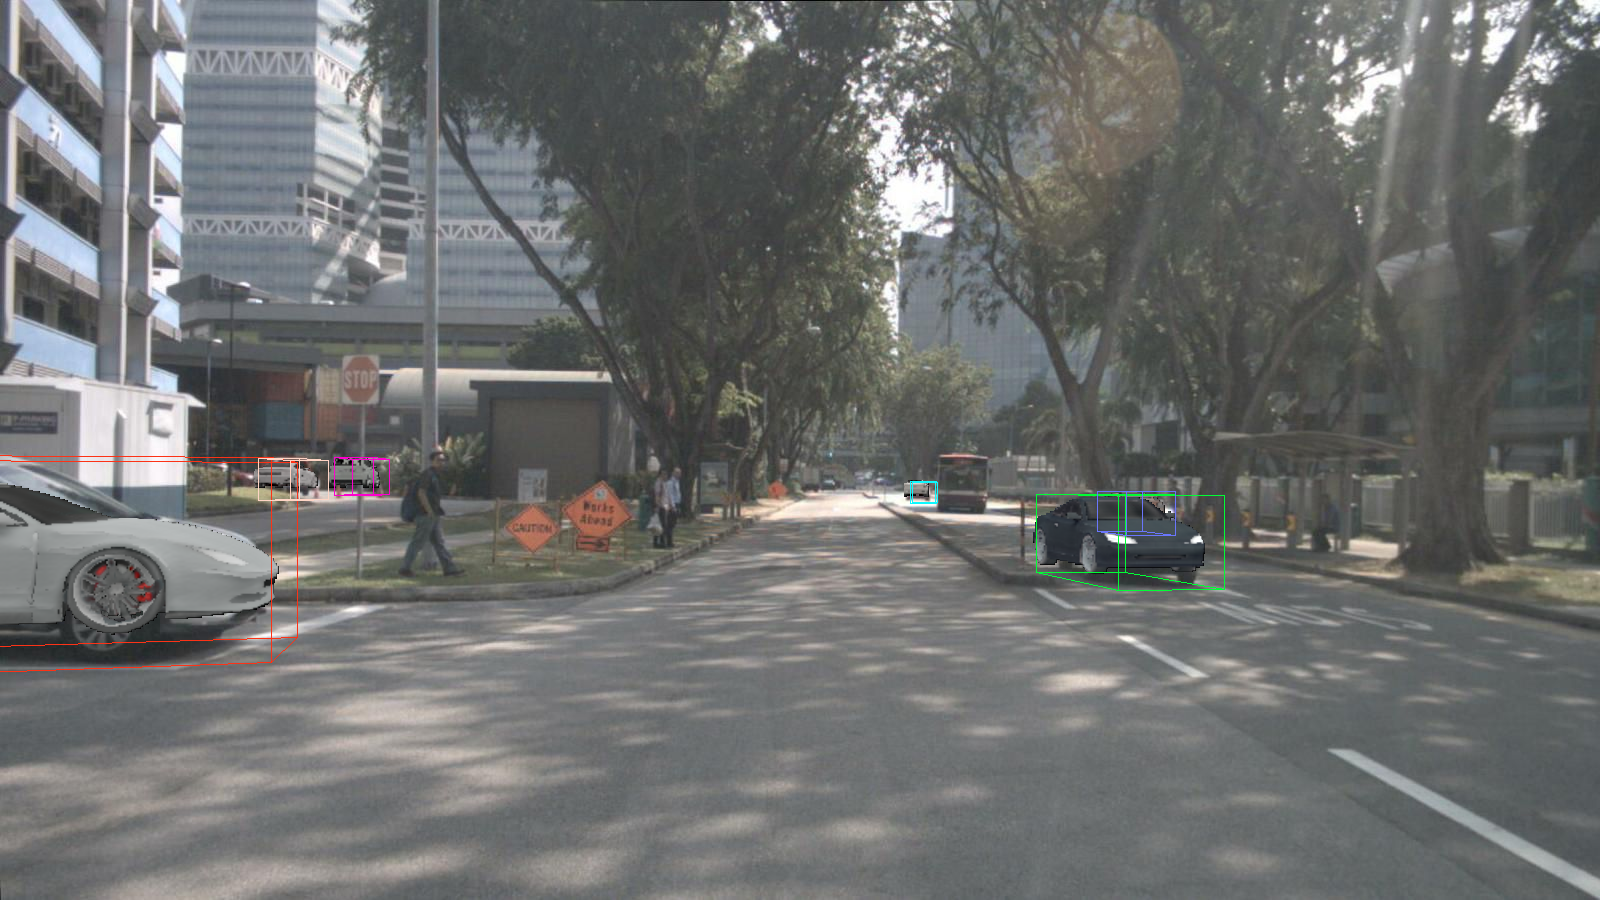
\includegraphics[width=.32\columnwidth, trim={0cm 0cm 0cm 0cm},clip]{fig/nuScenes_main/scene6/35_30_bbox.png}}&
		\raisebox{-0.5\height}{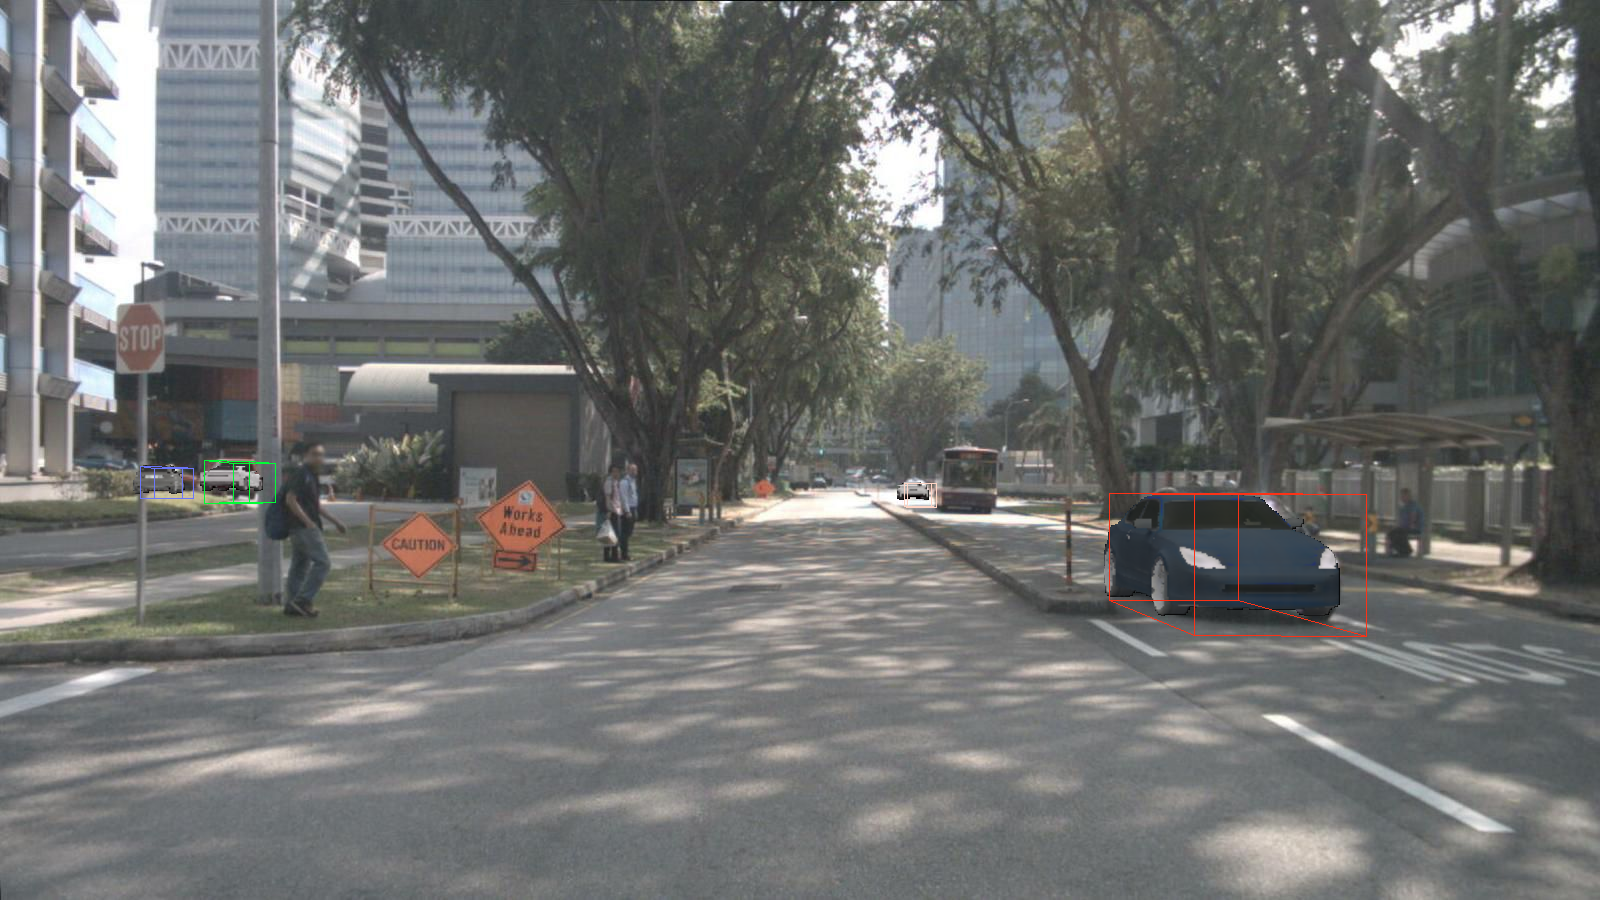
\includegraphics[width=.32\columnwidth, trim={0cm 0cm 0cm 0cm},clip]{fig/nuScenes_main/scene6/35_31_bbox.png}}\\[1.1cm]
  
            \rotatebox[origin=c]{90}{{\footnotesize	Parking lot}}&
  		\raisebox{-0.5\height}{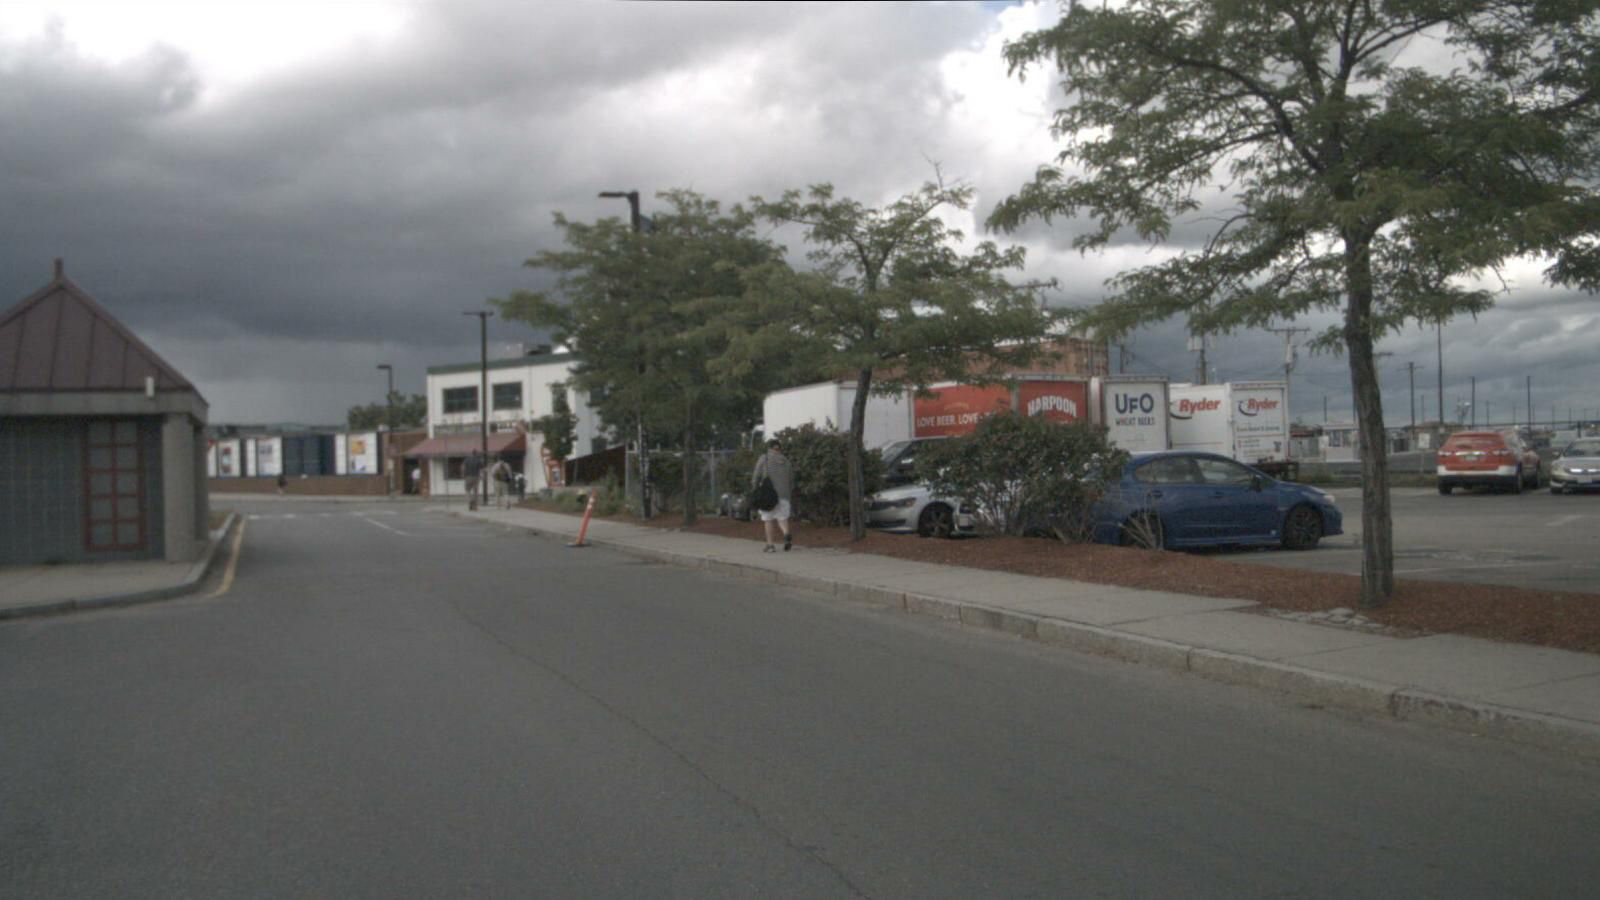
\includegraphics[width=.32\columnwidth, trim={0cm 0cm 0cm 0cm},clip]{fig/nuScenes_main/scene7/gt_2.png}}&
		\raisebox{-0.5\height}{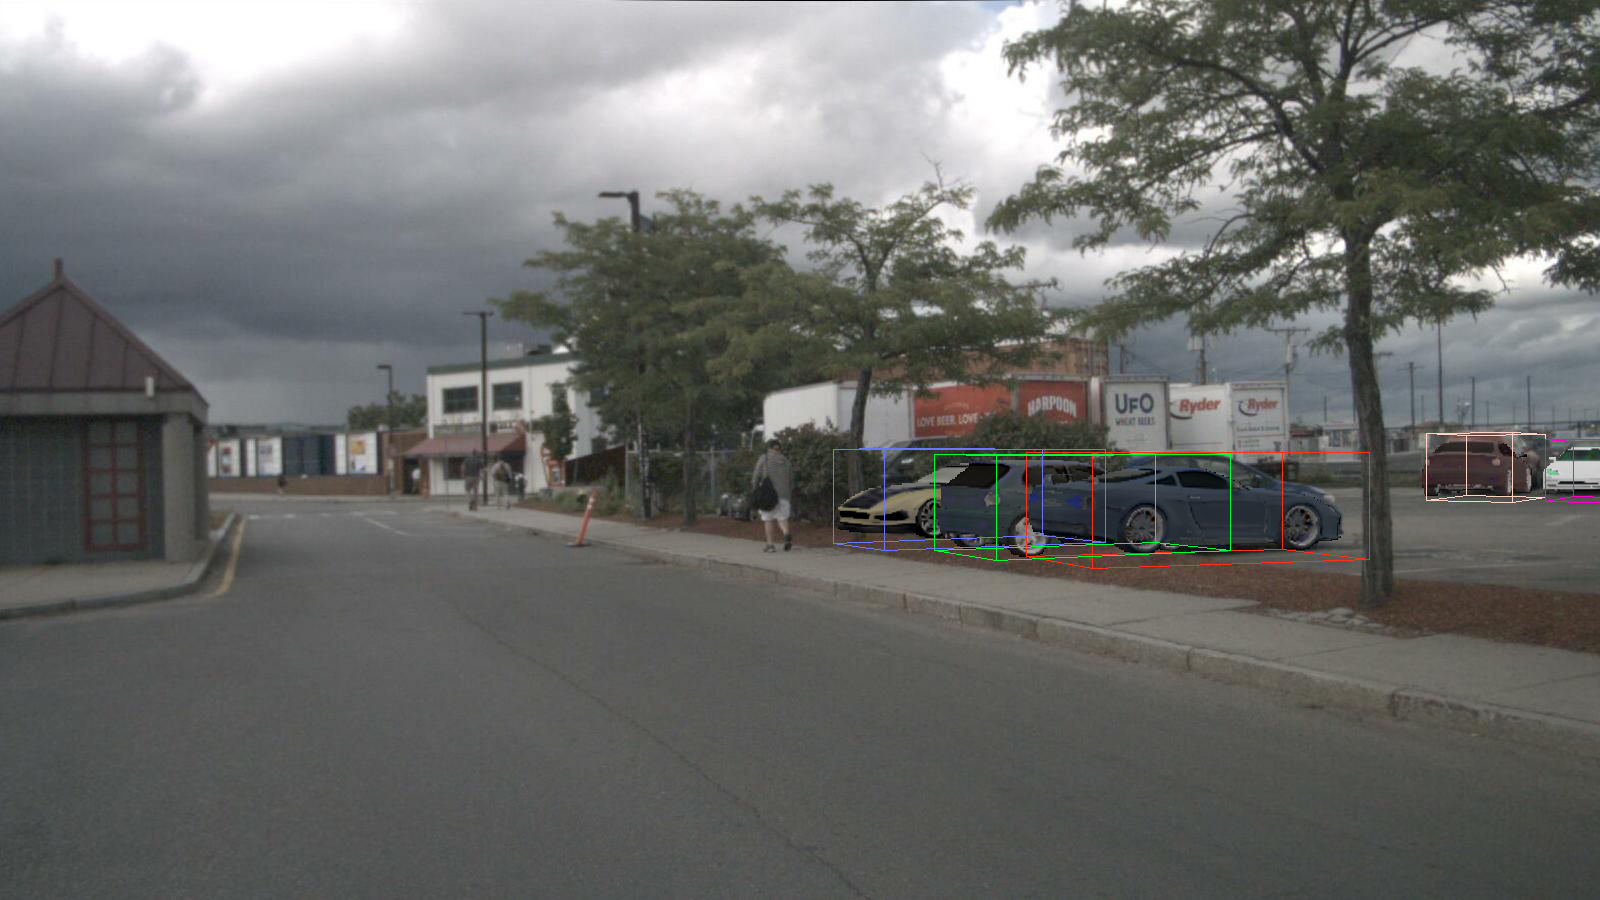
\includegraphics[width=.32\columnwidth, trim={0cm 0cm 0cm 0cm},clip]{fig/nuScenes_main/scene7/bbox_0.png}}&
		\raisebox{-0.5\height}{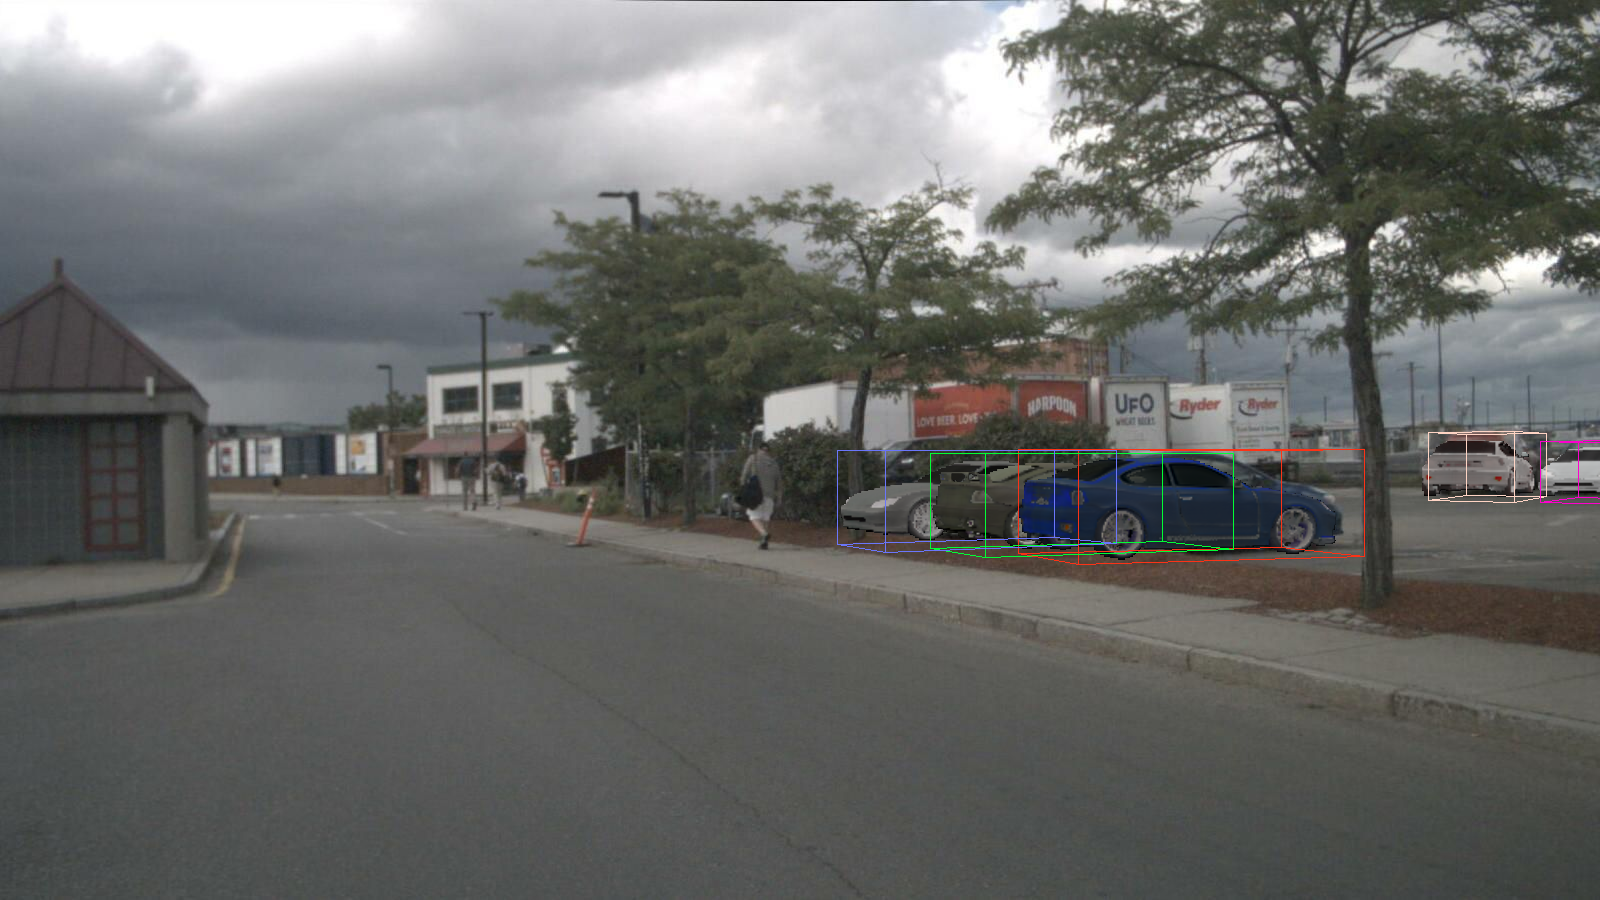
\includegraphics[width=.32\columnwidth, trim={0cm 0cm 0cm 0cm},clip]{fig/nuScenes_main/scene7/bbox_1.png}}&
		\raisebox{-0.5\height}{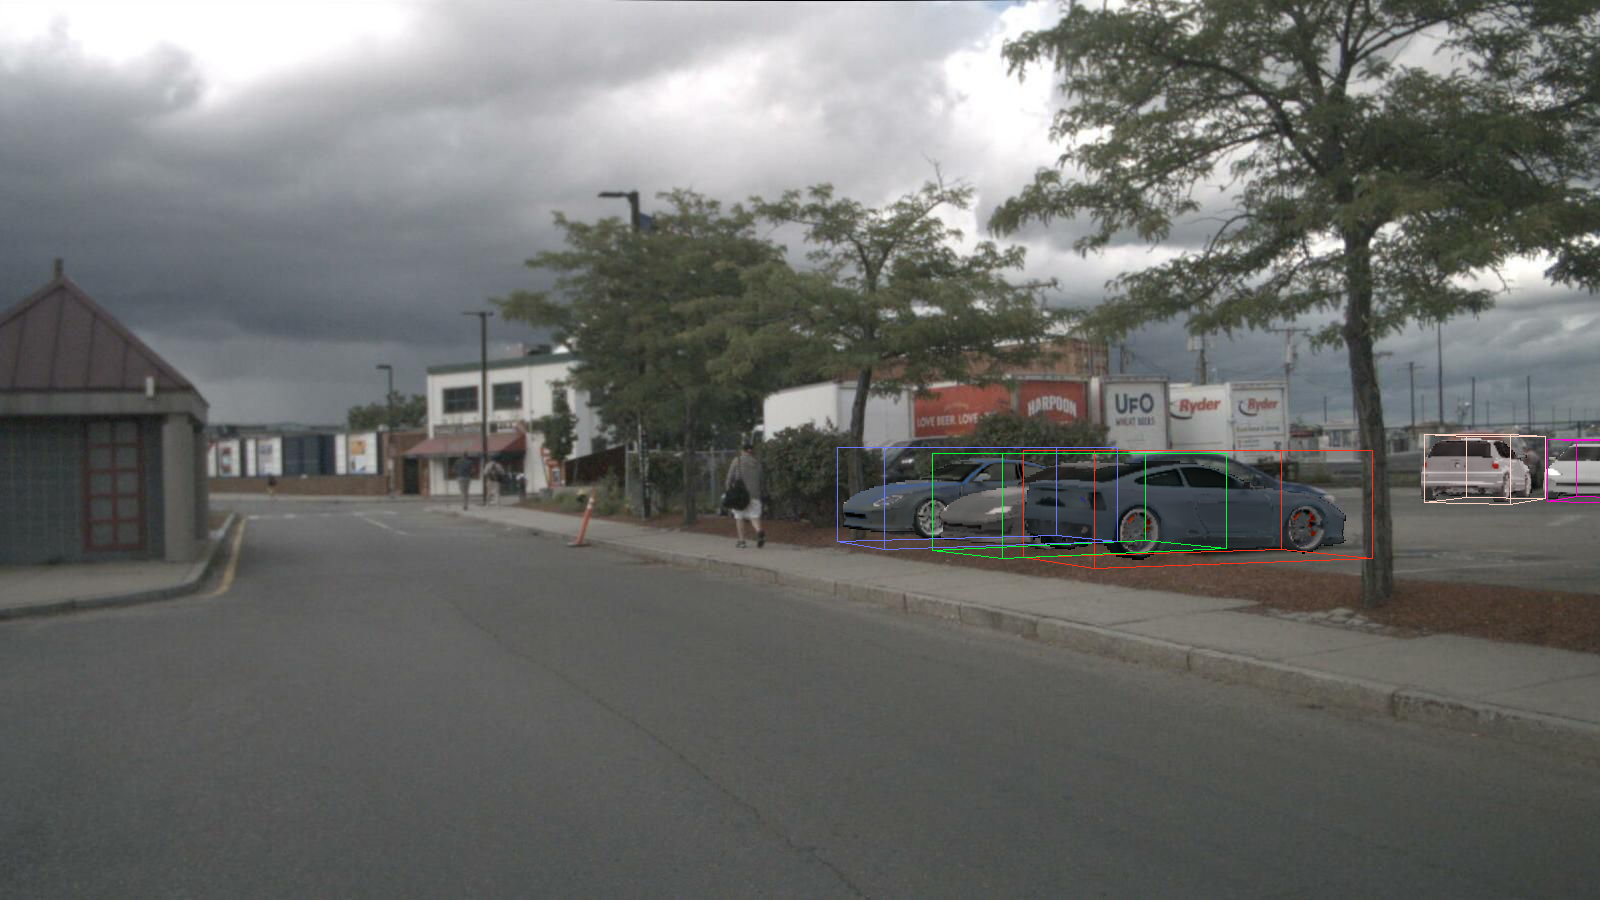
\includegraphics[width=.32\columnwidth, trim={0cm 0cm 0cm 0cm},clip]{fig/nuScenes_main/scene7/bbox_3.png}}&
		\raisebox{-0.5\height}{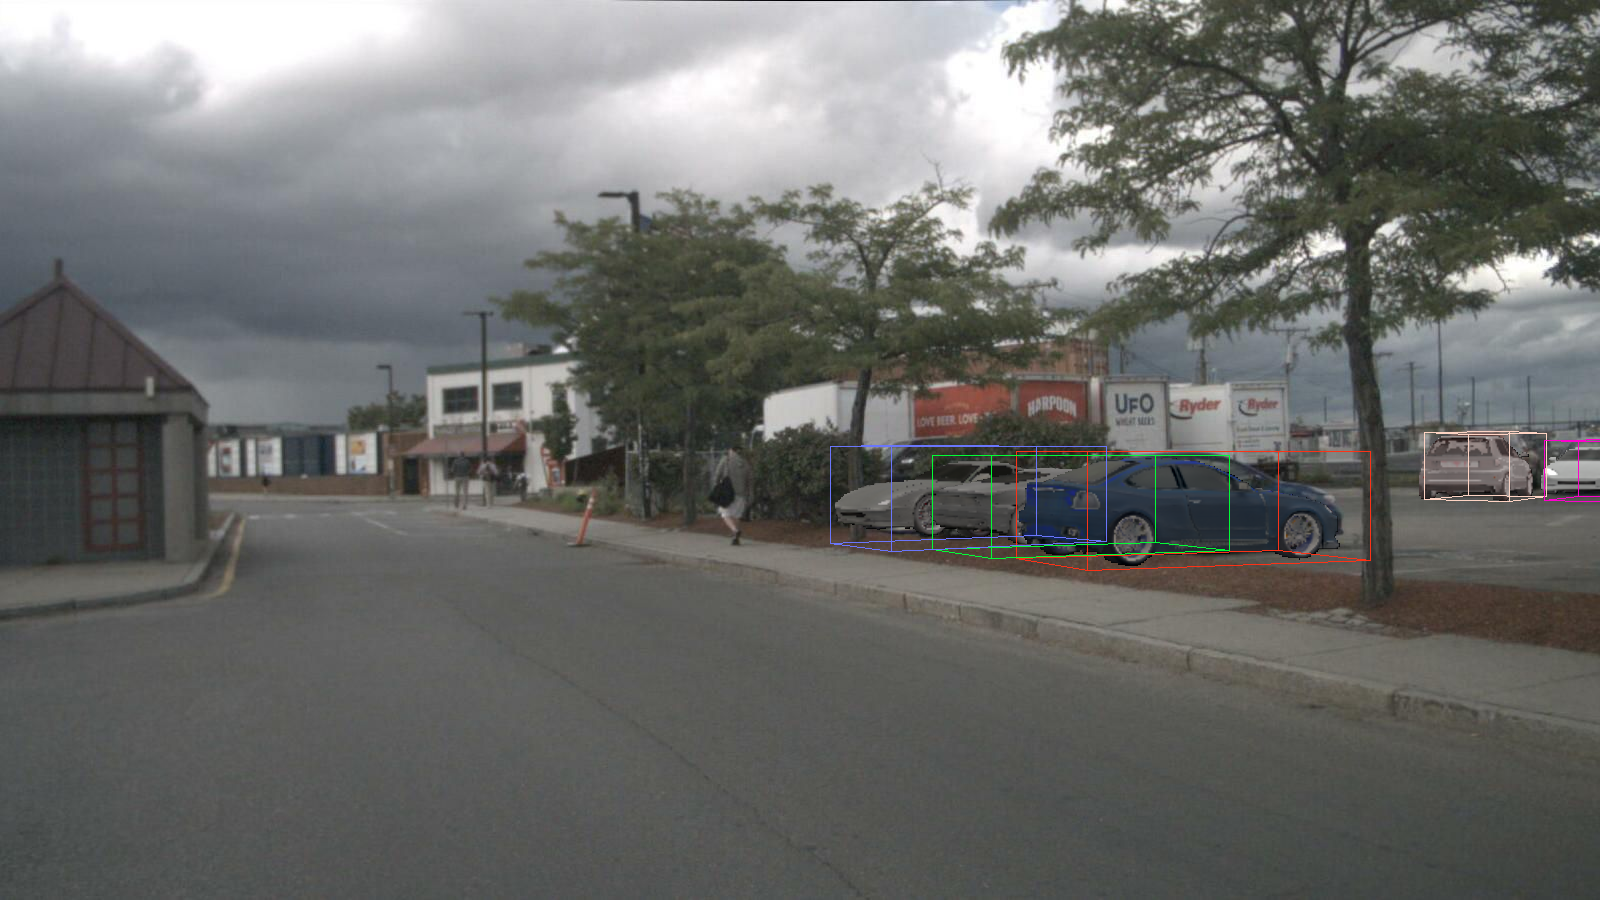
\includegraphics[width=.32\columnwidth, trim={0cm 0cm 0cm 0cm},clip]{fig/nuScenes_main/scene7/bbox_33.png}}\\%[0.95cm]
		
	\end{tabular}
	}
\vspace*{-6pt}
\caption{Tracking via Inverse Neural Rendering on nuScenes~\cite{caesar2020nuscenes}. From left to right, we show (i) observed images from diverse scenes at timestep $k=0$; (ii) an overlay of the optimized generated object and its 3D bounding boxes at timestep $k=0, 1, 2 \text{ and } 3$. The color of the bounding boxes for each object corresponds to the predicted tracklet ID. We see that even in such diverse scenarios, our method does not lose any tracks and performs robustly across all scenarios, although the dataset is unseen.}\label{fig:nuScenes_results}
\vspace*{-12pt}
\end{figure*}
\vspace{0.5\baselineskip} \noindent \textbf{Interpretable Latent Matching.}
%
% \todo{explain matching as IOU, embedding, geometry, and modality x distance}
In the matching stage, all optimal object representations $o_p$ in frame $k$ are matched with \emph{tracked} and \emph{lost} objects from $k-1$. Objects are matched based on appearance and location with a weighted affinity score
% \vspace*{-8pt}
\begin{equation}\label{eq:affinity}
    A = w_{IoU} A_{IoU,3D} + w_{z} A_{z} + w_{c} D_{centroid},
\end{equation}
where $A_{IoU,3D}$ is the IoU of the 3D boxes computed over the predictions of tracked object predictions $\mathbf{x}_{k|k-1}$ and refined observations. Here, the object affinity $A_{z}$ is computed as the cosine distance of tracked object latent embeddings $\mathbf{z}$. In addition to that the Euclidean distance between the center $D_{centroid}$ adds additional guidance. We add no score for unreasonable distant tracked objects and detections.

We compute the best combination of tracked and detected objects using the Hungarian algorithm~\cite{kuhn1955hungarian}, again a conventional choice in existing tracking algorithms. Matched tracklet and object pairs are kept in the set of \emph{tracked} objects and the representation of the corresponding detections is discarded, while unmatched detections are added as new objects.
Unmatched tracklets are set to \emph{lost} with a lost frame counter of one. Objects that were not detected in previous frames are set to \emph{tracked} and their counter is reset to $0$. Objects with a lost frame count higher than lifespan $N_{life}$, or outside of the visible field, are removed.


\vspace{0.5\baselineskip} \noindent \textbf{Track and Embedding Update.}
%
In the update step, we refine each object embedding $\mathbf{z}$  and motion model $\mathbf{y}_{k}$ given the result of the matching step. Embeddings are updated through an exponential moving average
\vspace*{-4pt}
\begin{equation}
    \mathbf{z}_{k, EMA}  = \beta \mathbf{z}_k + (1 - \beta) \mathbf{z}_{k-1, EMA}  \text{ with } \beta = \frac{2}{T-1}
\end{equation}
over all past observations of the object, where $T$ is the number of observed time steps of the respective instance. The observation $\mathbf{y}_{k}$ is used to update the Kalman filter. The optimal Kalman gain
\begin{equation}
   \mathbf{K}_{k} = \mathbf{P}_{k|k-1}\mathbf{H}^{T} ( \mathbf{H}\mathbf{P}_{k|k-1}\mathbf{H}^{T} + R)^{-1}
\end{equation}
is updated to minimize the residual error of the predicted model and the observation. The observation $\mathbf{y}_{k}$ is used to estimate the object state as
\begin{equation}
   \hat{\mathbf{x}}_{k|k} = \hat{\mathbf{x}}_{k|k-1} + \mathbf{K}_{k}(\mathbf{y}_{k} - \mathbf{H}\hat{\mathbf{x}}_{k|k-1}) 
\end{equation}
and with
\vspace*{-4pt}
\begin{equation}
   \mathbf{P}_{k} = \mathbf{P}_{k|k-1} - \mathbf{K}_k \mathbf{H}  \mathbf{P}_{k|k-1}
\end{equation}
the \textit{a posteriori} of the covariance matrix is updated.



% \subsection{Implementation Details}\label{ssec:optim}

% \subsubsection{Representation Model.} 
% We employ the GET3D~\cite{gao2022get3d} architecture as object model $G$. Following StyleGAN~\cite{karras2019styleGAN,karras2020styleGAN2} embeddings $z_{T}$ and $z_{S}$ are mapped to intermediate style embeddings $\boldmath{w}_S$ and $\boldmath{w}_T$ in a learned $\boldmath{W}\text{-space}$, which we optimize over instead of $\boldmath{Z}\text{-space}$. Style embeddings condition a generator function that produces tri-planes representing object shapes as Signed Distance Fields (SDFs) and textures as texture fields. We deliberately \emph{train our generator on synthetic data only}, see experiments below. Differentiable marching tetrahedra previously introduced in DMTet~\cite{shen2021dmtet} extract a mesh representation and Images are rendered with a differentiable rasterizer~\cite{laine2020modular}.

%\subsubsection{Generalization Across Domains.} 
%We deliberately \emph{train our generator on synthetic data only}. Specifically, we use ShapeNet~\cite{shapenet2015} for training and we find generalizable performance due to the specific perceptual similarity rather than accurate RGB. Evaluating the experiments in this work on unseen real-world datasets without fine-tuning, we find that the proposed tracking pipeline generalizes across different datasets and \emph{does not require any training.}  


% We use a pretrained checkpoint of the GET3D \cite{gao2022get3d} mesh-based generative model trained on synthetic images of cars from the ShapeNetv1 dataset \cite{shapenet2015} in our work. However, our method of optimizing over the latent space of an object representation can be generalized to any other generative representation model for cars. GET3D inherently disentangles texture and geometry by first mapping independently drawn Gaussian latent vectors $z_{T,p}$ and $z_{S,p}$ representing the texture and geometry respectively to a learned distribution to obtain $w_{tex}$ and $w_{geo}$, and then predicting the texture and geometry of the car via a shared CNN-based backbone. 
% method used are given in the implementation section and a review of  GET3D~\cite{gao2022get3d} and marching tetrahedras~\cite{shen2021dmtet} is provided in the supplementary.




%TODO: We probably don't have space for a tracking algorithm in the main paper. Would need to move to the supplement.
%\begin{algorithm}
%  \caption{Tracking algorithm \todo{Remove placeholder and tracking algorithm}}\label{algo:tracking}
%  \begin{algorithmic}[1]
%    \Procedure{Euclid}{$a,b$}\Comment{The g.c.d. of a and b}
%      \State $r\gets a\bmod b$
%      \While{$r\not=0$}\Comment{We have the answer if r is 0}
%        \State $a\gets b$
%        \State $b\gets r$
%        \State $r\gets a\bmod b$
%      \EndWhile\label{euclidendwhile}
%      \For{\texttt{<some condition>}}
%        \State \texttt{<do stuff>}
%      \EndFor
%      \State \textbf{return} $b$\Comment{The gcd is b}
%    \EndProcedure
%  \end{algorithmic}
%\end{algorithm}

